\documentclass[ExampleMasters.tex]{subfiles}
\begin{document}

	\chapter{APPENDIX D}
	{\Large Model Validation}

	\section{Introduction}
	The vehicle model described in the preceeding chapter was tested extensively and trends in vehicle performance parameters corresponding to specific variable parameters were sought as a means of validating the model and certifying it worthy of use in the optimisation solver. The findings from the analysis of the longitudinal modeling of the long vehicle combination structure with additional electric propulsion on specific axles are presented here. The design variables, or model parameters, in this analysis include the following:
	\begin{itemize}
	\item Gross Combination Weight (GCW)
	\item Axle loads on propelled axles
	\item Engine size
	\item Electric Machine sizing / rating
	\item Electric buffer capacity and operating range
	\item Buffer State of Charge (SoC) management
	\end{itemize}
	Broadly listed, the output signals / parameters are as follows:
	\begin{itemize}
	\item Mission time
	\item Fuel consumption
	\item Charge consumption patterns over the mission and total charge consumed
	\item Combination startability
	\item Minimum combination speed at high gradients (alternatively, combination gradeability at specific speeds)
	\item Mission productivity
	\item Percentage of the mission that is power limited in operation nature
	\item Percentage of the mission that is traction / grip limited in operation nature
	\end{itemize}
	\section{Vehicle model and simulation}
	In all cases, the long combination considered is the standard A-Double, consisting of a 6X4 tractor (Unit 1), 3-axle semitrailer (Unit 2), 2-axle dolly (Unit 3) and another 3-axle semitrailer (Unit 4), in order. Specific combinations were chosen to demonstrate the influence of the model parameters on the outputs and these results are documented in this report. The A-Double propulsion configurations used for analysis were the following:
	\begin{itemize}
	\item Pure Combustion combination - 011-000-00-000
	\item One axle on the first semitrailer propelled - 011-010-00-000
	\item One axle each on the first semitrailer and dolly propelled - 011-010-01-000
	\item One axle each on all three trailing units propelled - 011-010-01-010
	\item All axles on all three trailing units propelled - 011-111-11-111
	\end{itemize}
	The GCWs considered are 50t, 60t, 70t and 80t. The axle/unit loading in each case is listed in Table \ref{table:unitLoads}.
	\begin{table}[ht]
	\caption{Individual unit loads}
	\centering
	\begin{tabular}{c c c c c}
	\hline\hline
	Unit number & GCW=50t & GCW=60t & GCW=70t & GCW=80t \\
	\hline
	1 & 18080 & 18420 & 22434 & 22434\\
	2 & 15100 & 20100 & 22100 & 22400\\
	3 & 7000 & 8000 & 10500 & 12500 \\
	4 & 10000 & 13480 & 13480 & 22400 \\
	\hline
	\end{tabular}
	\label{table:unitLoads}
	\end{table}
	The axle propulsion configuration of a specific combination is represented as in the below example.
	Combination 011-010-00-001 indicates:
	\begin{itemize}
	\item Axle 1 dead, Axles 2 and 3 propelled in Unit 1
	\item Axle 1 and 3 dead, Axle 2 propelled in Unit 2
	\item Both Axles 1 and 2 dead in Unit 3
	\item Axles 1 and 2 dead, Axle 3 propelled in Unit 4
	\end{itemize}
	The mission selected for validation and optimisation is G\"oteborg-Malm\"o, spanning a distance of approximately 294 km. The gradient profile of the route is shown in Figure \ref{roadGradient}.
	\begin{figure}
	\centering
	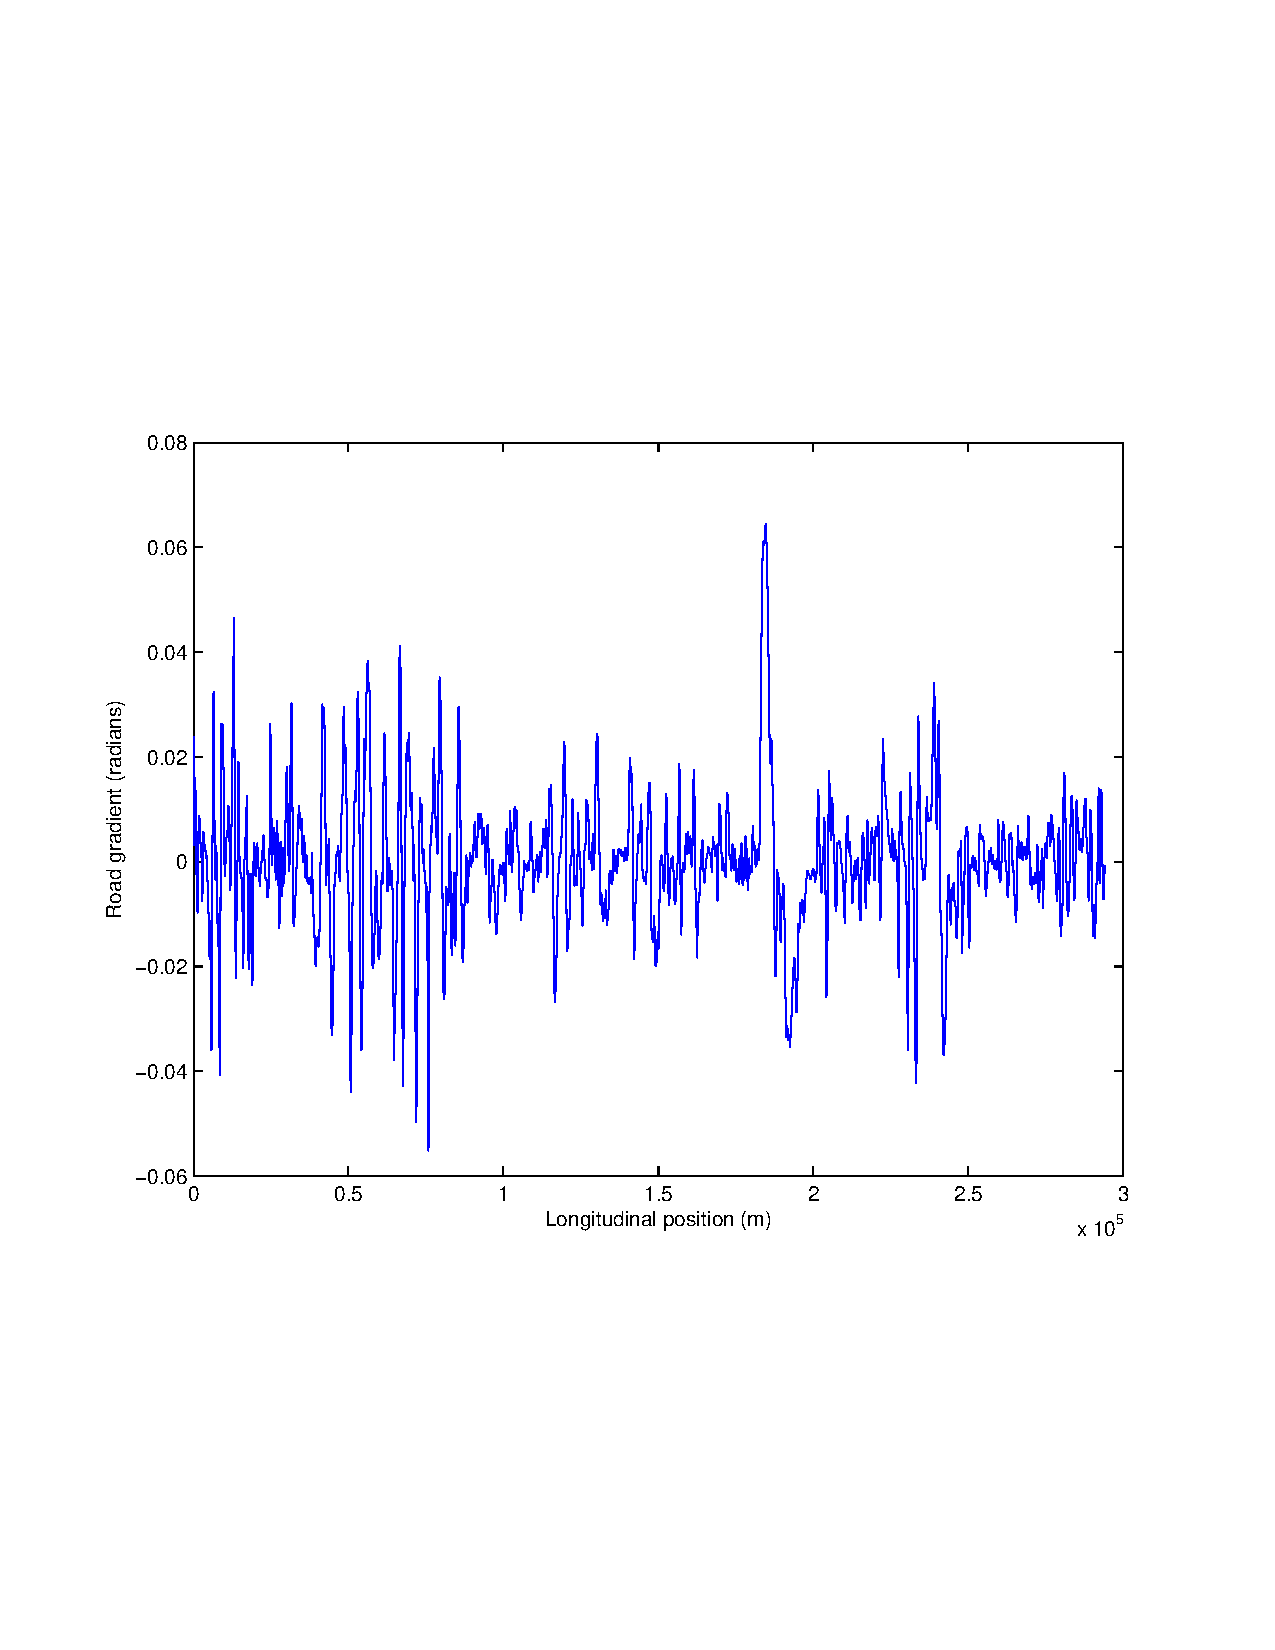
\includegraphics[width=80mm, clip=true, trim=45 185 65 208]{figures/ModelValidation/PlotsWithNonPredictiveControl/roadGradient.pdf}
	\caption{Road gradient vs longitudinal position}
	\label{roadGradient}
	\end{figure}
	The engines used for simulating the tractive machine in the tractor are the D11K450 EU6, D13C540 EU5 and D16G750 EU5 Volvo engines. The electric motors used are of ratings 120kW \& 230Nm, 173kW \& 411Nm and 180kW \& 420Nm. The electric buffers used on each unit are of capacities 4976640, 6272640 and 5987500 Coulombs. The simulation whose results are dealt with below involved a constant target speed of 80kmph throughout the mission.\\
	The upper and lower bounds on the buffer state of charge can either be pre-set or dynamically altered during the course of the mission. The decision to place these bounds is often drawn from prior knowledge of impending assistive use of electrical energy based on varying gradients, vehicle speeds and other traction-influencing factors. Three different energy management strategies were employed in the validation and the optimal strategy was chosen to be used in the optimisation.
	\begin{itemize}
	\item Constant depth of discharge
	\item Non-predictive pre-set varying depths of discharge along the mission
	\item Fully predictive preset varying depths of discharge
	\end{itemize}
	The strategy and the model results for each of the above are presented in the forthcoming section. Results are presented in subsections, each pertaining to a specific model parameter's role in the vehicle performance. For example, the effect of increasing gross combination weight keeping the axle propulsion configuration and engine size constant is discussed in a single subsection.
	\section{Constant depth of discharge}
	The simplest control strategy is to place fixed maximum and minimum buffer State of Charge (SoC) limits irrespective of instantaneous elevation and forthcoming gradients or changes in vehicle set speed. In this case, the minimum and maximum buffer SoC values were set at 0.3 and 1 respectively, corresponding to 30\% and 100\% of the buffer's total charge capacity. The lack of correspondence to road gradient makes the buffer availability susceptible to changes disproportionate to vehicle energy requirements. There thus exists the possibility of the buffer being drained completely before a steep ascent or the buffer being fully charged before an impending descent. Since the knowledge of the mission remains unutilised, vehicle performance with this strategy can be expected to be sub-optimal.
	\subsection{Engine Size and GCW}
	The combination propelled \textit{solely by the tractor combustion engine} was tested first to observe the effects of the engine size and gross combination weight on the mission performance. As expected, for a given engine, mission time and fuel consumption increases with increasing GCW as shown in Figure \ref{timeFuelGCWEngine}. Increasing the GCW from 50t to 80t showed a 39\% increase in fuel consumption for the D11 and D13 engine powered combinations and a 36\% increase in fuel consumption for the D16 engine powered combination. The percentage increase in mission times for the D11, D13 and D16 engine powered combinations was 2.56\%, 1.71\% and 1.36\% respectively.

	\begin{figure}
	\begin{subfigure}{.5\textwidth}
	\centering
	\includegraphics[width=\linewidth, clip=true, trim=45 185 65 208]{figures/ModelValidation/PlotsWithNonPredictiveControl/EngineSizeAndGCW/FuelConsumptionVsGCWAndEngineSize.pdf}
	\caption{Fuel consumption over mission}
	\end{subfigure}
	\begin{subfigure}{.5\textwidth}
	\centering
	\includegraphics[width=\linewidth, clip=true, trim=45 185 65 210]{figures/ModelValidation/PlotsWithNonPredictiveControl/EngineSizeAndGCW/MissionTimeVsGCWAndEngineSize.pdf}
	\caption{Mission time}
	\end{subfigure}
	\caption{Effect of engine size and GCW on fuel consumption and mission time}
	\label{timeFuelGCWEngine}
	\end{figure}
	\begin{figure}
	\centering
	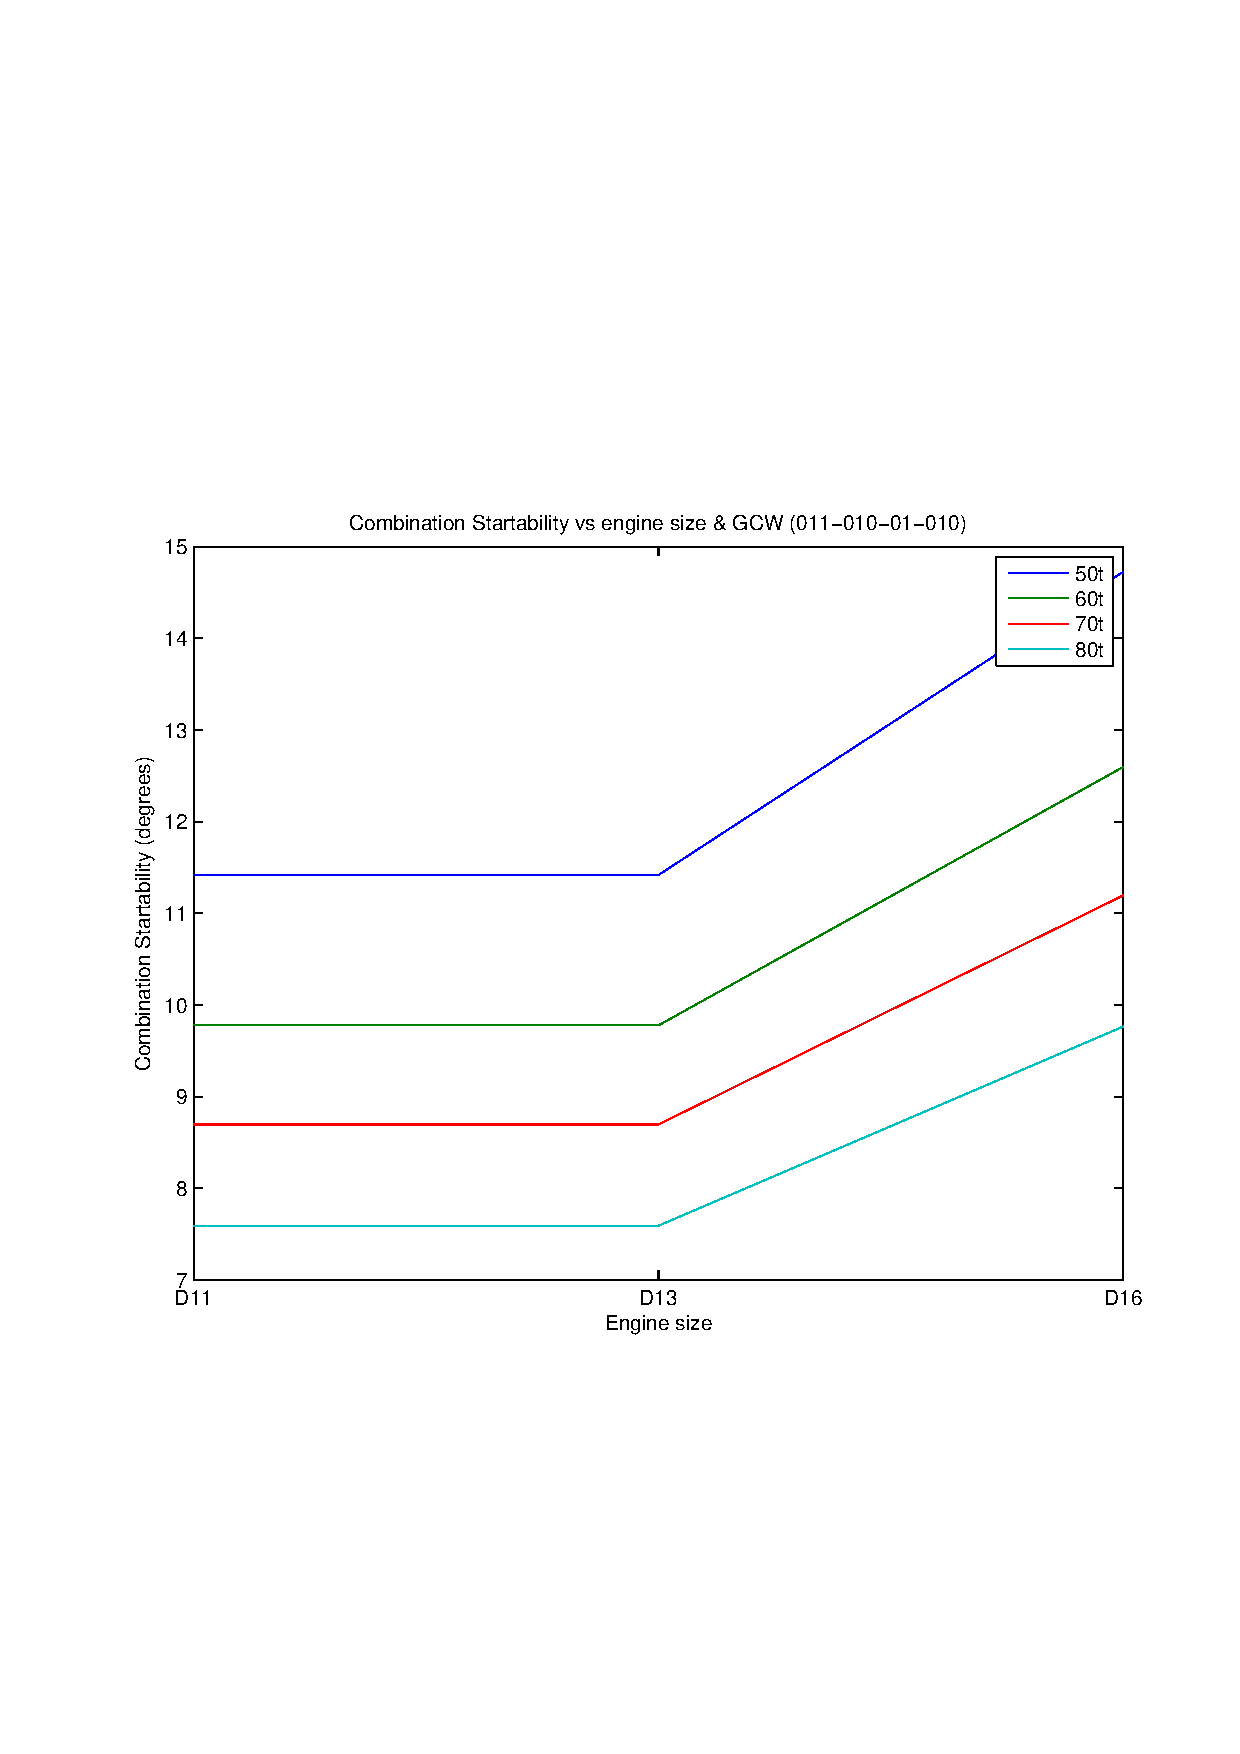
\includegraphics[width=0.5\linewidth, clip=true, trim=45 185 65 208]{figures/ModelValidation/PlotsWithNonPredictiveControl/EngineSizeAndGCW/CombinationStartabilityVsGCWAndEngineSize.pdf}
	\caption{Effect of engine size and GCW on combination startability}
	\label{startabilityEngineGCW}
	\end{figure}
	It should be noted here that the D13 engine shows higher fuel economy than the D11 and D16 engines for the same GCW. The startability of the combinations was also similarly compared as depicted in Figure \ref{startabilityEngineGCW}. Since the combination is traction limited at lower GCWs, the startability is unaffected by engine size for GCWs 50t and 60t. The unchanged startability at higher GCWs between the D11 and D13 combinations can be attributed to the similar starting torques (close to idling engine RPM) of the two engines. It must be noted that this comparison benefits from identical tractor rear axle loads. The influence of axle load on the startability will be examined in a later section.
	\begin{figure}
	\centering
	\includegraphics[width=\linewidth, clip=true, trim=45 185 65 208]{figures/ModelValidation/PlotsWithNonPredictiveControl/EngineSizeAndGCW/MissionSpeedVsPosition.pdf}
	\caption{Effect of engine size and GCW on combination speed along the mission}
	\label{missionSpeedEngineSizeGCW}
	\end{figure}
	\begin{figure}
	\begin{subfigure}{.5\textwidth}
	\centering
	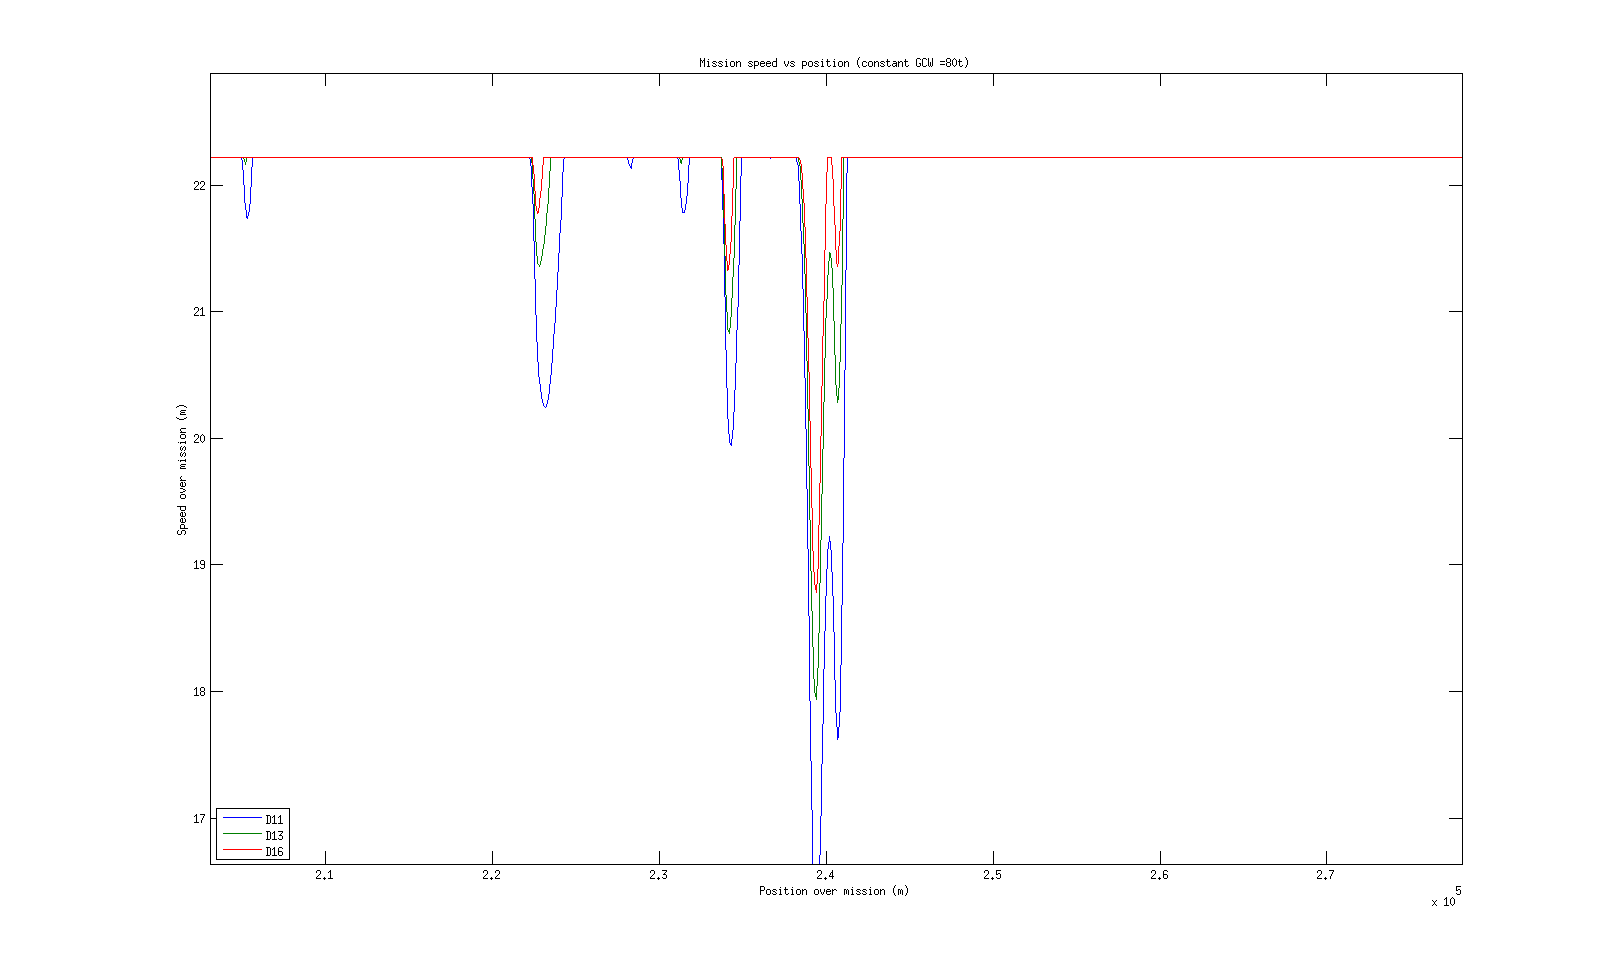
\includegraphics[width=\linewidth]{figures/ModelValidation/PlotsWithNonPredictiveControl/EngineSizeAndGCW/MissionSpeed80tZoomed.png}
	\caption{D11 has significantly lower average speeds}
	\end{subfigure}
	\begin{subfigure}{.5\textwidth}
	\centering
	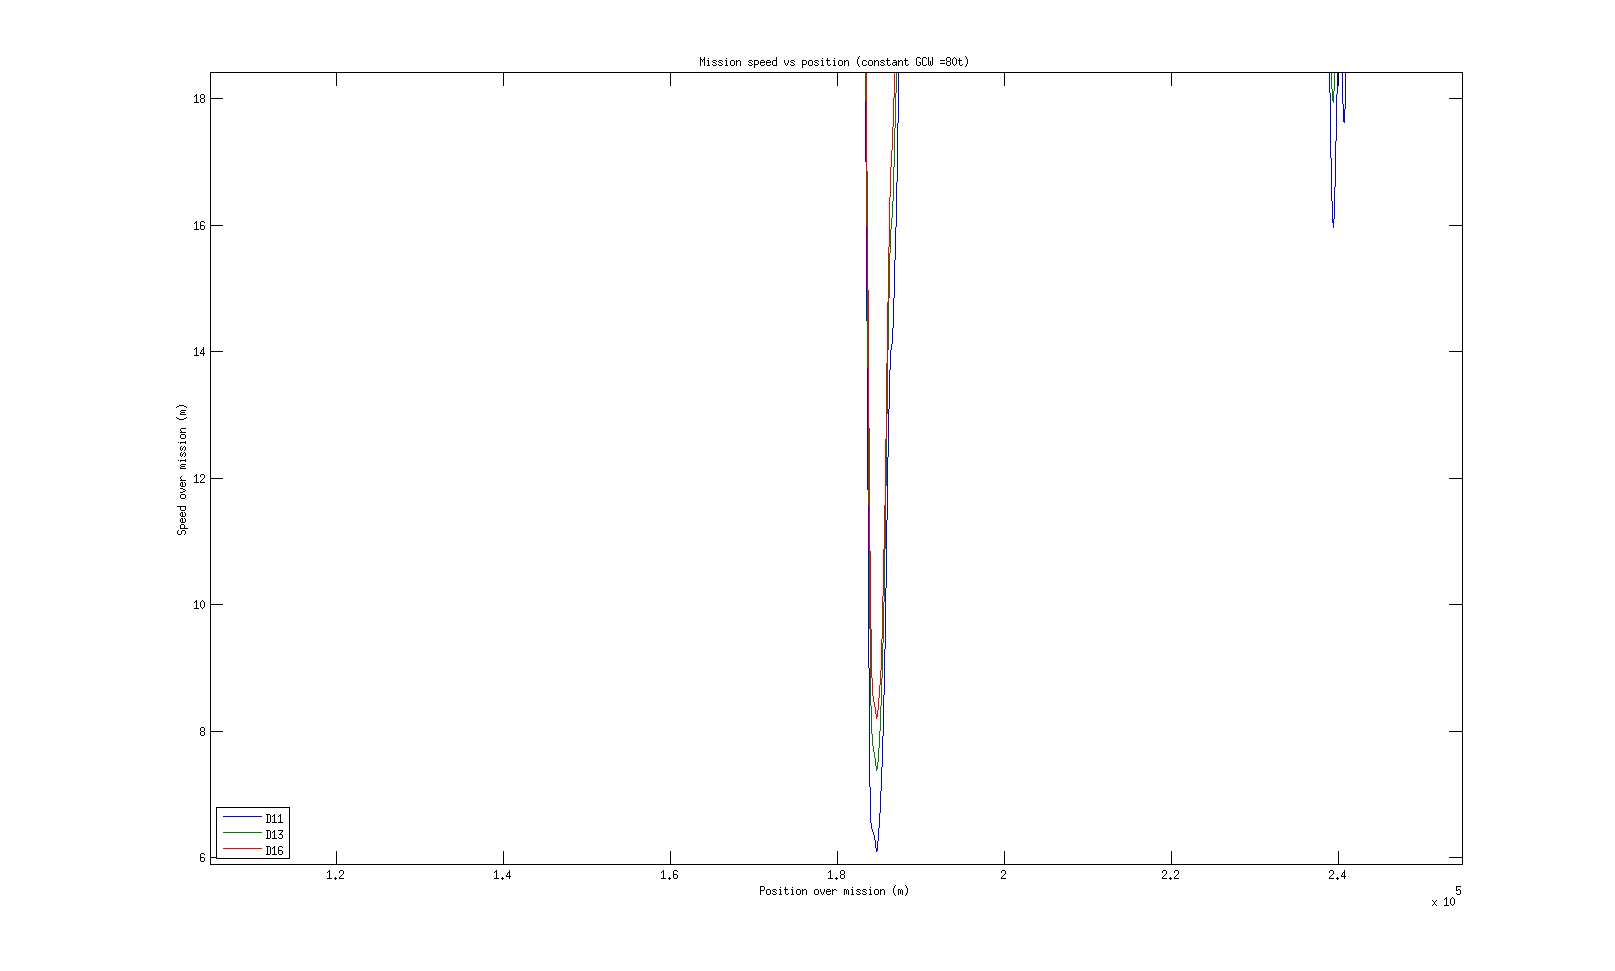
\includegraphics[width=\linewidth]{figures/ModelValidation/PlotsWithNonPredictiveControl/EngineSizeAndGCW/MissionSpeed80tZoomedMaxGradient.png}
	\caption{Speed at max altitude (Hallands\aa sen)}
	\end{subfigure}
	\caption{Effect of engine size and GCW on combination speed along the mission}
	\label{zoomedMissionSpeedEngineSizeGCW}
	\end{figure}
	The speed of the combination along the mission is then recorded and compared among the three engines. This is depicted for all loads in Figure \ref{missionSpeedEngineSizeGCW}. As can be seen, the maximum speed at the top of the highest gradient along the mission reduces with increasing GCW and with engine downsizing. At higher loads, much of the mission along gradients is power limited. The gap in combination performance is hence accentuated at higher loads. A zoomed in view of the combination speed for the combination of GCW 80t is shown in Figure \ref{zoomedMissionSpeedEngineSizeGCW}. The speeds at the crest of the gradient are 7.11ms\textsuperscript{-1}, 8.59ms\textsuperscript{-1} and 9.59ms\textsuperscript{-1} for the combinations powered by the D11, D13 and D16 engines respectively.\\
	The combination with the D11 engine thus decelerates the most, up the gradient at Hallands\aa sen. It can also be seen from the plots that the combination with D16 engine begins deceleration the latest and quickly recovers the target speed thus maintaining a sizeably higher average speed over the D11 and D13 combinations.
	\subsection{Number of axles propelled}
	The conundrum of increasing the number of propelled axles correlates directly with the axle load distribution and road surface. Hence, increasing propulsive power improves mission startability and average speed only upto a point beyond which the traction limits of the road make the excess power unusable. This progressive improvement and the performance cusp is investigated here. The common GCW considered is 68t.

	\begin{figure}
		\begin{subfigure}{.5\textwidth}
			\centering
			\includegraphics[width=\linewidth, clip=true, trim=45 185 65 208]{figures/ModelValidation/PlotsWithNonPredictiveControl/IncreasingNumberOfAxles/FuelConsumptionVsAxleNumberAndEngineSize.pdf}
			\caption{Fuel consumption over mission}
		\end{subfigure}
		\begin{subfigure}{.5\textwidth}
			\centering
			\includegraphics[width=\linewidth, clip=true, trim=45 185 65 210]{figures/ModelValidation/PlotsWithNonPredictiveControl/IncreasingNumberOfAxles/MissionTimeVsAxleNumberAndEngineSize.pdf}
			\caption{Mission time}
		\end{subfigure}
		\caption{Effect of number of propelled axles \& engine size on fuel consumption and mission time}
		\label{timeFuelNumberOfAxlesEngine}
	\end{figure}

	It can be noticed here, as depicted in Figure \ref{timeFuelNumberOfAxlesEngine}, taking the D13 combination in specific, that the fuel consumption reduces while increasing the number of propelled axles to 1 and 2 consecutively. Thereafter, additional propulsion adversely affects fuel consumption, though, of course, staying significantly below the pure combustion combination. This anomaly can be explained by observing that the charge availability is erratic and often non-existent during ascents / positive gradients as can be seen in Figure \ref{SoCVsPosition} where the buffer SoC is at its minimum just before the steep ascent at Hallands\aa sen. This shifts the tractive load onto the engine effectively defeating the purpose of adding electric propulsion to more trailer axles. The earlier observation of the energy management strategy being sub-optimal stands vindicated. The percentage reductions in fuel consumption are tabulated in Table \ref{table:fuelConsumptionReductionAxles}.
	\begin{figure}
	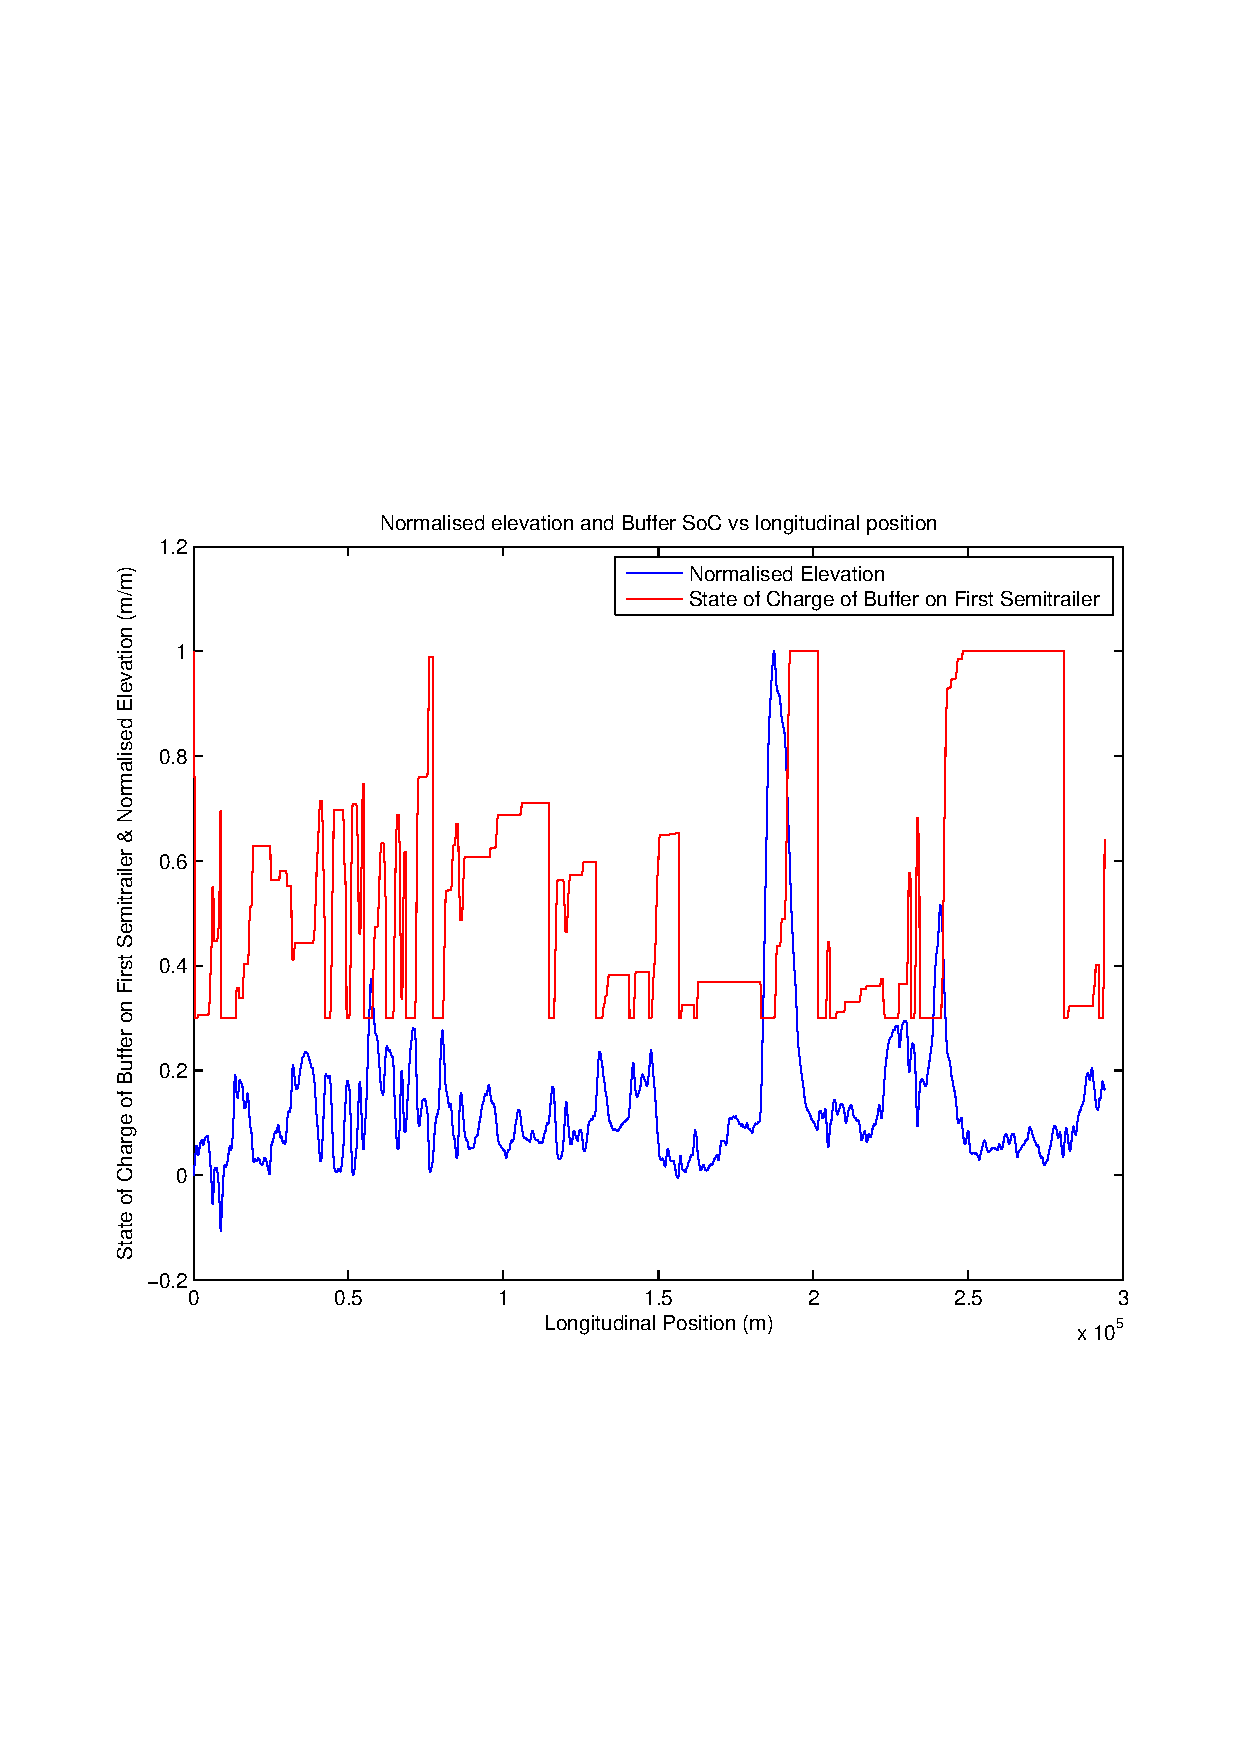
\includegraphics[width=\textwidth,clip=true, trim=45 180 45 190]{figures/ModelValidation/PlotsWithNonPredictiveControl/IncreasingNumberOfAxles/SoCVsElevation.pdf}
	\caption{Normalised elevation and corresponding Buffer SoC vs longitudinal position}
	\label{SoCVsPosition}
	\end{figure}
	The mere addition of a single electrically propelled axle (173kW \& 411Nm electric motor for each propelled axle and 5.98MC buffer for each respective unit) on the D11 engine-only combination yields a 6.2\% reduction in fuel consumption while the potential savings are significantly improved in the case of the D13 combinations. Savings of upto 9.9\% compared to the engine-only combinations are seen with the addition of one propelled axle each on every trailing unit. Observing the trends in the D16 combinations clearly show successive increases in fuel consumption upto a point where the engine optimum operation trend mitigates the savings to around 3\%. This substantiates the motivation rendered earlier.
	\begin{table}
	\centering
	\begin{tabular}{|c|c|c|c|c|c|c|}
	\hline
	& 011-010-00-000 & 011-010-01-000 & 011-010-01-010 & 011-011-01-010 & 011-011-11-010 \\
	\hline
	D11 & 6.17 & 6.31 & 5.89 & 6.17 & 5.52 \\
	\hline
	D13 & 5.69 & 6.81 & 9.9 & 5.09 & 4.56 \\
	\hline
	D16 & 2.19 & 3.1 & 3.34 & 2.84 & 2.89 \\
	\hline
	\end{tabular}
	\caption{Percentage reduction in fuel consumption compared to standard A-Double}
	\label{table:fuelConsumptionReductionAxles}
	\end{table}
	\begin{figure}
	\centering
	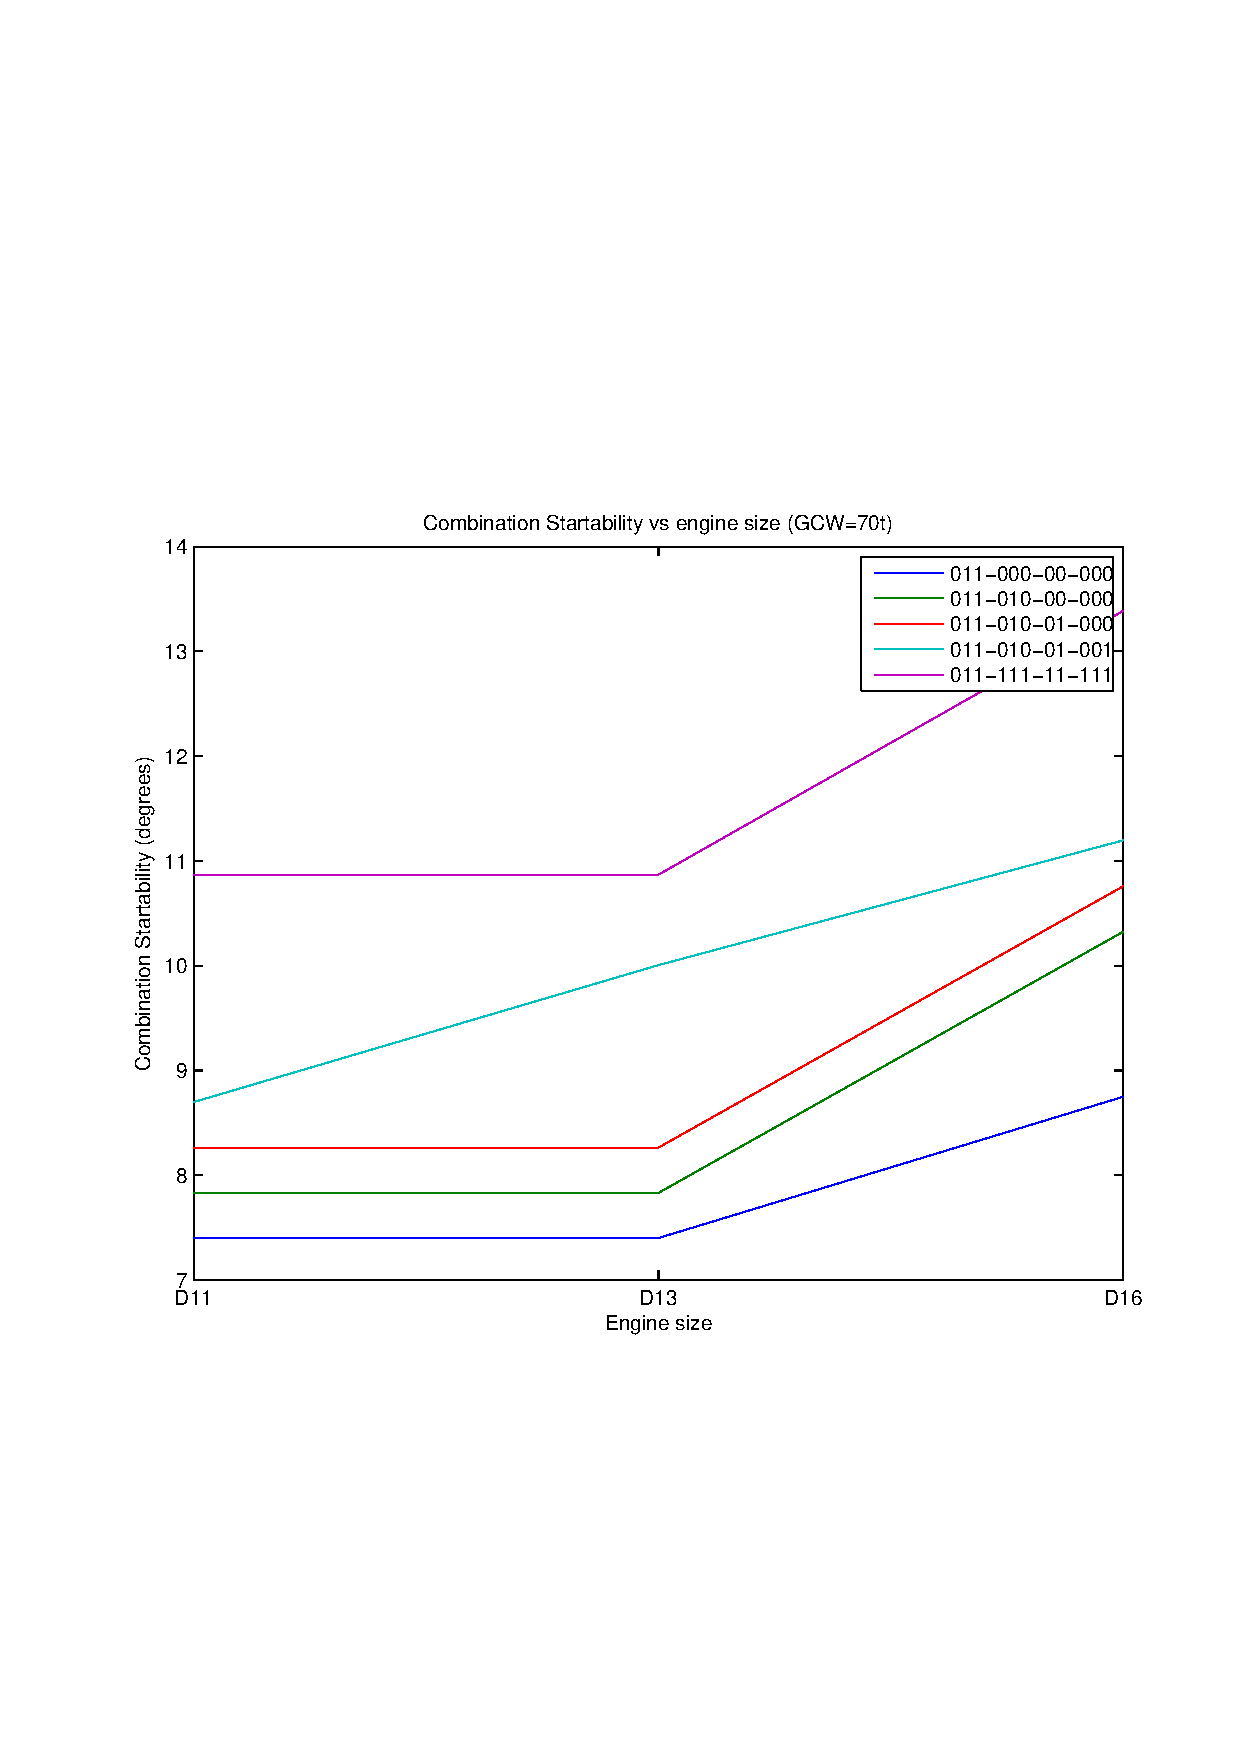
\includegraphics[width=0.5\linewidth, clip=true, trim=45 185 65 208]{figures/ModelValidation/PlotsWithNonPredictiveControl/IncreasingNumberOfAxles/CombinationStartabilityVsAxleNumberAndEngineSize.pdf}
	\caption{Effect of engine size and number of propelled axles on combination startability}
	\label{startabilityEngineNumberOfAxles}
	\end{figure}
	The startability of the combination is analysed in a manner similar to before to establish the effect of increased tractive power and is as shown in Figure \ref{startabilityEngineNumberOfAxles}. It must be noted that the rating of the electric motors was maintained constant while simulation combinations with increased number of propelled axles. Hence, the addition of electric machines to the combination results in equally spaced steps on increased startability. Also, as stated before, the identical starting torques of the D11 and D13 engines coupled with the use of similar motors results in the startability of the two combinations remaining similar in each propelled axle configuration case.\\
	With a constant GCW of 70t, the effect of increasing electric propulsion on the mission speed is shown in Figure \ref{globalMissionSpeedIncreasedPropulsion}. The delay in the beginning of combination deceleration with increased propulsion and the increased minimum speed at the peak of Hallands\aa sen is clearly seen in Figure \ref{missionSpeedIncreasedPropulsion}. While the pure combustion combination achieves a speed of 9.45ms\textsuperscript{-1}, the addition of one electrically propelled axle increases this speed to 10.42ms\textsuperscript{-1} which is further improved to 11.22ms\textsuperscript{-1} with the addition of another electrically propelled axle. It must be noted that this increase in minimum speed alone cannot be directly attributed to the addition of propulsion since the traction available uphill also depends on the buffer states and efficiencies. Nevertheless, while the buffers are 'available' in this segment, the effect of addition of propulsion while evident upto two axles added, is almost unseen with successive addition of axles owing to inefficient use of buffer electrical energy as discussed earlier. The charge consumption in each of the cases is shown in Figure \ref{chargeEngineSizeNumberOfAxles}.
	\begin{figure}
	\centering
	\includegraphics[width=0.5\linewidth, clip=true, trim=45 185 65 208]{figures/ModelValidation/PlotsWithNonPredictiveControl/IncreasingNumberOfAxles/ChargeConsumptionVsAxleNumberAndEngineSize.pdf}
	\caption{Effect of engine size and number of propelled axles on charge consumption}
	\label{chargeEngineSizeNumberOfAxles}
	\end{figure}
	\begin{figure}
	\centering
	\includegraphics[width=\linewidth, clip=true, trim=45 185 65 200]{figures/ModelValidation/PlotsWithNonPredictiveControl/IncreasingNumberOfAxles/MissionSpeedVsPosition(constantGCW70t).pdf}
	\caption{Increased propulsion and its influence on mission speed}
	\label{globalMissionSpeedIncreasedPropulsion}
	\end{figure}
	\begin{figure}
	\begin{subfigure}{.5\textwidth}
	\centering
	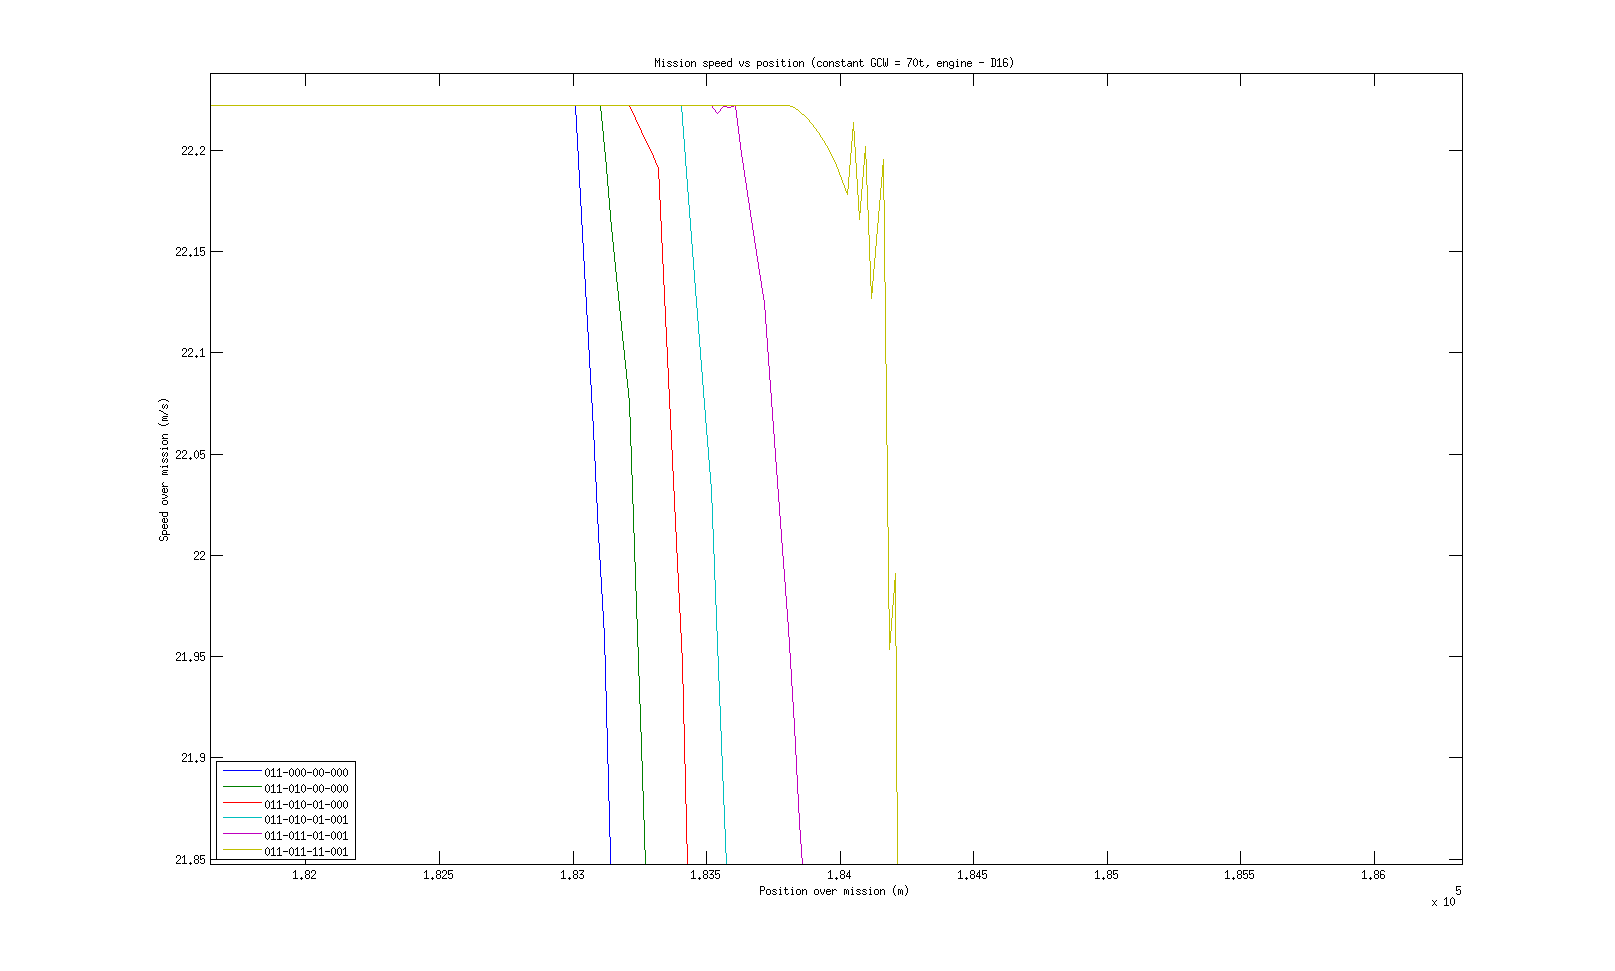
\includegraphics[width=\linewidth]{figures/ModelValidation/PlotsWithNonPredictiveControl/IncreasingNumberOfAxles/SpeedVsPositionZoomedNoOfAxlesBeginDec.png}
	\caption{Vehicle speed at the beginning of Hallands\aa sen}
	\end{subfigure}
	\begin{subfigure}{.5\textwidth}
	\centering
	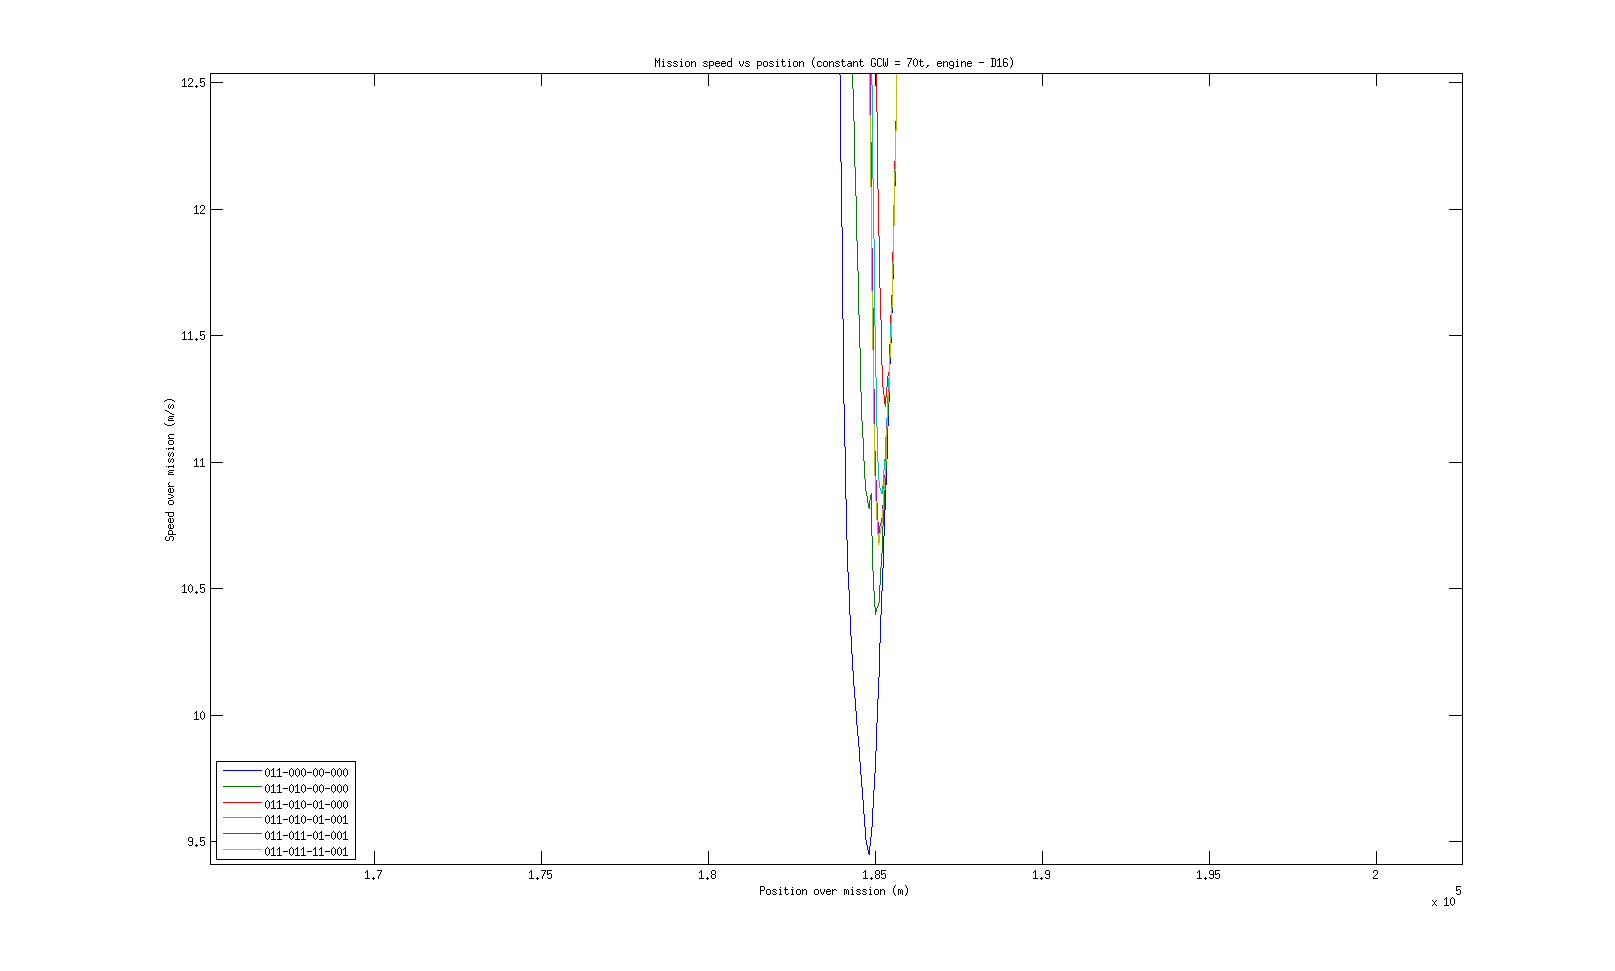
\includegraphics[width=\linewidth]{figures/ModelValidation/PlotsWithNonPredictiveControl/IncreasingNumberOfAxles/SpeedVsPositionZoomedNoOfAxlesPeak.png}
	\caption{Speed at the peak of Hallands\aa sen}
	\end{subfigure}
	\caption{Effect of number of propelled axles on mission speed}
	\label{missionSpeedIncreasedPropulsion}
	\end{figure}
	\subsection{Axle load}
	The axle load of propelled axles determines the useability of the traction that the motor provides. When presented with the problem of choosing a specific number or combination of axles to be propelled given a specified number of electric machines, the choice of axles must be preferential with higher axle loads. This is inspected by assigning an electric machine alternatively to three different axles with varying axle loads and observing the mission performance. Each axle on the first semitrailer, dolly and the second semitrailer in the A-Double combination carry 7.3t, 5.25t and 4.49t respectively. Hence, in each of the simulations performed, a single axle on one of the three trailing units is chosen to be propelled. A constant GCW of 70t is assigned.\\
	The fuel consumption and mission time in each of the cases is depicted in Figure \ref{fuelTimeEngineAxleLoad}.
	\begin{figure}
	\begin{subfigure}{.5\textwidth}
	\centering
	\includegraphics[width=\linewidth, clip=true, trim=45 185 65 206]{figures/ModelValidation/PlotsWithNonPredictiveControl/EffectOfAxleLoad/FuelConsumptionVsAxleLoadAndEngineSize.pdf}
	\caption{Fuel consumption over mission}
	\end{subfigure}
	\begin{subfigure}{.5\textwidth}
	\centering
	\includegraphics[width=\linewidth, clip=true, trim=45 185 65 206]{figures/ModelValidation/PlotsWithNonPredictiveControl/EffectOfAxleLoad/MissionTimeVsAxleLoadAndEngineSize.pdf}
	\caption{Mission time}
	\end{subfigure}
	\caption{Effect of axle load on fuel consumption and mission time}
	\label{fuelTimeEngineAxleLoad}
	\end{figure}
	The seemingly curious unchanged fuel consumption and mission times across axle loads for the D11 and D13 engines can be explained by analysing the axle loads in conjunction with power limited operation mode. In the D11 and D13 combinations, even in cases when the tractive force demand was limited by the friction limits of the tire and road, the required power more often than not exceeded the maximum power that the engine and motors could independently produce. This can be seen by comparing the percentage of the mission that the combination was traction limited (as shown in Table \ref{table:tractionLimitMode}) to that when the combination was power limited (as shown in Table \ref{table:powerLimitMode}). In the case of the D16 combinations, when electric propulsion is added to the axle carrying the least load (4.5t), the tractive force demand being grip limited results in the combination being power limited for a smaller fraction of the mission allowing the engine to operate at its optimum point thereby leading to a smaller fuel consumption. The total charge consumption over the mission in each of the cases in shown in Figure \ref{chargeEngineSizeAxleLoad}.
	\begin{figure}
	\centering
	\includegraphics[width=0.5\linewidth, clip=true, trim=45 185 65 208]{figures/ModelValidation/PlotsWithNonPredictiveControl/EffectOfAxleLoad/ChargeConsumptionVsAxleNumberAndAxleLoad.pdf}
	\caption{Effect of engine size and axle load on charge consumption}
	\label{chargeEngineSizeAxleLoad}
	\end{figure}
	\begin{table}
	\centering
	\begin{tabular}{|c|c|c|c|}
	\hline
	& Axle Load 7.4t & Axle Load 5.25t & Axle Load 4.5t \\
	& 011-010-00-000 & 011-000-01-000 & 011-000-00-010 \\
	\hline
	D11 & 5.31 & 5.63 & 5.75 \\
	\hline
	D13 & 3.01 & 3.13 & 3.17 \\
	\hline
	D16 & 2.10 & 2.18 & 1.79 \\
	\hline
	\end{tabular}
	\caption{Percentage of the mission that was traction-limited}
	\label{table:tractionLimitMode}
	\end{table}
	\begin{table}
	\centering
	\begin{tabular}{|c|c|c|c|}
	\hline
	& Axle Load 7.4t & Axle Load 5.25t & Axle Load 4.5t \\
	& 011-010-00-000 & 011-000-01-000 & 011-000-00-010 \\
	\hline
	D11 & 10.85 & 10.85 & 10.84 \\
	\hline
	D13 & 5.64 & 5.64 & 5.64 \\
	\hline
	D16 & 5.53 & 5.53 & 4.34 \\
	\hline
	\end{tabular}
	\caption{Percentage of the mission operating in power-limit mode}
	\label{table:powerLimitMode}
	\end{table}
	The startability of the combinations can thus be analysed in a similar manner and is depicted in Figure \ref{startabilityEngineAxleLoad}.\\
	\begin{figure}
	\centering
	\includegraphics[width=0.5\linewidth, clip=true, trim=45 185 65 208]{figures/ModelValidation/PlotsWithNonPredictiveControl/EffectOfAxleLoad/CombinationStartabilityVsAxleLoadAndEngineSize.pdf}
	\caption{Effect of engine size and axle load on combination startability}
	\label{startabilityEngineAxleLoad}
	\end{figure}
	\subsection{Machine power / torque rating}
	Combined with the axle load problem is one of choosing the right electric machine rating for the axle. The effect of the machine rating is direct in that the torque available at the axle is varied by the choice of the rating. The D13 engine powered 011-010-00-000 combination with a GCW of 70t is chosen for this exercise. The combination is simulated with varying electric machine ratings. The fuel consumption and mission time in each of the cases is depicted in Figure \ref{fuelTimeEngineAxleLoad}.
	\begin{figure}
	\begin{subfigure}{.5\textwidth}
	\centering
	\includegraphics[width=\linewidth, clip=true, trim=45 185 65 206]{figures/ModelValidation/PlotsWithNonPredictiveControl/EffectOfMachinePowerRating/FuelConsumptionVsMachinePowerRating.pdf}
	\caption{Fuel consumption over mission}
	\end{subfigure}
	\begin{subfigure}{.5\textwidth}
	\centering
	\includegraphics[width=\linewidth, clip=true, trim=45 185 65 206]{figures/ModelValidation/PlotsWithNonPredictiveControl/EffectOfMachinePowerRating/MissionTimeVsMachinePowerRating.pdf}
	\caption{Mission time}
	\end{subfigure}
	\caption{Effect of machine power rating on fuel consumption and mission time}
	\label{fuelTimeEngineAxleLoad}
	\end{figure}
	The reduction in fuel consumption arising from additionally available electric propulsion is clearly seen in Figure \ref{fuelTimeEngineAxleLoad}. A fuel saving of 5.4\% is obtained from using the 180kW, 420Nm motor in place of the 120kW, 230Nm one. Also, the combination speed at the peak of Hallands\aa sen is improved by close to 2.5ms\textsuperscript{-1} from 8.59ms\textsuperscript{-1} to 11.05ms\textsuperscript{-1} as can be seen in Figure \ref{speedMissionMachineRating}. The choice of the machine rating is of course beset with the heavier costs associated with the machine and its auxiliaries. The productivity of the mission hence includes both these factors. Also, the reduced payload carrying capacity that results from higher rated machines being heavier is also factored while calculating mission revenues for mission productivity.

	\begin{figure}
	\centering
	\includegraphics[width=\linewidth, clip=true, trim=45 185 65 208]{figures/ModelValidation/PlotsWithNonPredictiveControl/EffectOfMachinePowerRating/MissionSpeedVsPosition(01101001010D13GCW70t).pdf}
	\caption{Effect of machine power rating on vehicle speed over mission}
	\label{speedMissionMachineRating}
	\end{figure}
	\subsection{Engine downsizing}
	The effect of downsizing the combustion engine on combinations with electrically propelled trailer axles is key to reducing mission costs and improving fuel economy thereby doubling boosting mission productivity. The 011-010-01-010 combination with a GCW of 70t is chosen and the combustion engine size is varied to observe the trends in fue consumption and mission time among other combination parameters.
	\begin{figure}
	\begin{subfigure}{.5\textwidth}
	\centering
	\includegraphics[width=\linewidth, clip=true, trim=45 185 65 206]{figures/ModelValidation/PlotsWithNonPredictiveControl/EngineDownsizing/FuelConsumptionVsEngineSize.pdf}
	\caption{Fuel consumption over mission}
	\end{subfigure}
	\begin{subfigure}{.5\textwidth}
	\centering
	\includegraphics[width=\linewidth, clip=true, trim=45 185 65 206]{figures/ModelValidation/PlotsWithNonPredictiveControl/EngineDownsizing/MissionTimeVsEngineSize(GCW70t).pdf}
	\caption{Mission time}
	\end{subfigure}
	\caption{Effect of engine downsizing on fuel consumption and mission time}
	\label{fuelTimeEngineDownsize}
	\end{figure}
	\begin{figure}
	\centering
	\includegraphics[width=0.5\linewidth, clip=true, trim=45 185 65 208]{figures/ModelValidation/PlotsWithNonPredictiveControl/EngineDownsizing/CombinationStartabilityVsEngineSize.pdf}
	\caption{Effect of engine downsizing on combination startability}
	\label{startabilityEngineDownsize}
	\end{figure}
	The benefits of choosing the D13 engine over the D16 engine merely based on the fuel economy and comparable mission time is evident, as can be seen in Figure \ref{fuelTimeEngineDownsize}. As expected, the startability of the 70t combination is advantaged by increasing engine size and is shown in Figure \ref{startabilityEngineDownsize}. It must be noted that since the mission times are comparable in case of the D13 and D16 engines, the advantage gained through increased gradeability over Hallands\aa sen and improved average speeds is inconsequential over the mission. The improved fuel economy for the given mission can also be traced to the fact that the percentage of the mission that is power limited in both cases (D13 and D16) is similar at 2.47\% and 3.9\% respectively.\\
	This observation is significant as it justifies the use of smaller engines combined with additional electric propulsion in order to be able to utilise gradient-derived potential energy more efficiently in place of fuel-derived energy. The case for choosing smaller engines owing to them being less expensive and lighter is also thus motivated.\\
	As expected, the drop in vehicle speed at gradients is more significant in the case of the smaller engine as can be seen in Figure \ref{speedEngineDownsizing}.
	\begin{figure}
	\centering
	\includegraphics[width=0.8\linewidth, clip=true, trim=45 185 65 208]{figures/ModelValidation/PlotsWithNonPredictiveControl/EngineDownsizing/MissionSpeedVsPosition(01101001010GCW70t).pdf}
	\caption{Effect of engine downsizing on vehicle speed over mission}
	\label{speedEngineDownsizing}
	\end{figure}
	Thus, as can be seen, while most of the trends in the output signals conform to expectations, the role of the energy management strategy in the efficiency of electrical energy usage is proved beyond doubt. This naturally leads to the decision to modify the method in which the lower and upper bounds of the buffer SoCs are assigned.
	\section{Fully-predictive pre-set varying depths of discharge}
	A predictive SoC management strategy utilises the knowledge of upcoming gradient changes and appropriately modifies the depth of discharge of each buffer. The strategy and its implementation is explained in detail in Appendix C. The improvement in the combination performance based on specific vehicle parameters is described in the following subsections.
	\subsection{Engine Size and GCW}
	The combination with one axle on each trailer electrically propelled (011-010-01-010) is simulated over the mission to investigate the effect of increasing GCW and engine size on vehicle output parameters. The buffer capacity on each unit is 6.3MC and the rating of the electric machine used on each propelled axle is 173kW, 411Nm. The trends in fuel consumption and mission time are as shown in Figure \ref{timeFuelGCWEnginePredictiveSoC}. The fuel consumption trends are in stark comparison to Figure \ref{timeFuelGCWEngine} with the D11 engine showing the best fuel economy over the mission with predictive SoC management. Across the range of GCWs and engine sizes, the gross fuel consumption values have reduced in comparison with the fixed SoC case and so have mission times. These indicate more efficient use of the electric machines owing to the predictive SoC management. It must be remembered, nevertheless, that merely fuel consumption or mission time are not indicators of better executed mission and productivity values as defined in Chapter 2 can only be valied measures of comparison.
	\begin{figure}
	\begin{subfigure}{.5\textwidth}
	\centering
	\includegraphics[width=\linewidth, clip=true, trim=45 185 55 208]{figures/ModelValidation/PlotsWithPredictiveControl/EngineSizeAndGCW/FuelConsumptionVsGCWAndEngineSize.pdf}
	\caption{Fuel consumption over mission}
	\end{subfigure}
	\begin{subfigure}{.5\textwidth}
	\centering
	\includegraphics[width=\linewidth, clip=true, trim=45 185 55 210]{figures/ModelValidation/PlotsWithPredictiveControl/EngineSizeAndGCW/MissionTimeVsGCWAndEngineSize.pdf}
	\caption{Mission time}
	\end{subfigure}
	\caption{Effect of engine size and GCW on fuel consumption and mission time with predictive SoC control}
	\label{timeFuelGCWEnginePredictiveSoC}
	\end{figure}
	The speed of the combination over the mission for each of the four chosen GCWs is plotted for the combination with the D13 engine in Figure \ref{speedEngineDownsizingPredictiveSoC}. The clear improvement in minimum speed at the peak of Hallands\aa sen with reduction in GCW as opposed to the aberrant trends seen in Figure \ref{zoomedMissionSpeedEngineSizeGCW} is further proof of the efficacy of utilising the knowledge of the mission to regulate SoC limits.
	\begin{figure}
	\centering
	\includegraphics[width=0.6\linewidth, clip=true, trim=45 185 50 208]{figures/ModelValidation/PlotsWithPredictiveControl/EngineSizeAndGCW/MissionSpeedVsPosition(constantGCW=70t,engine-D13).pdf}
	\caption{Vehicle speed over mission - 011-010-01-010, D13, 70t}
	\label{speedEngineDownsizingPredictiveSoC}
	\end{figure}
	\begin{figure}
	\centering
	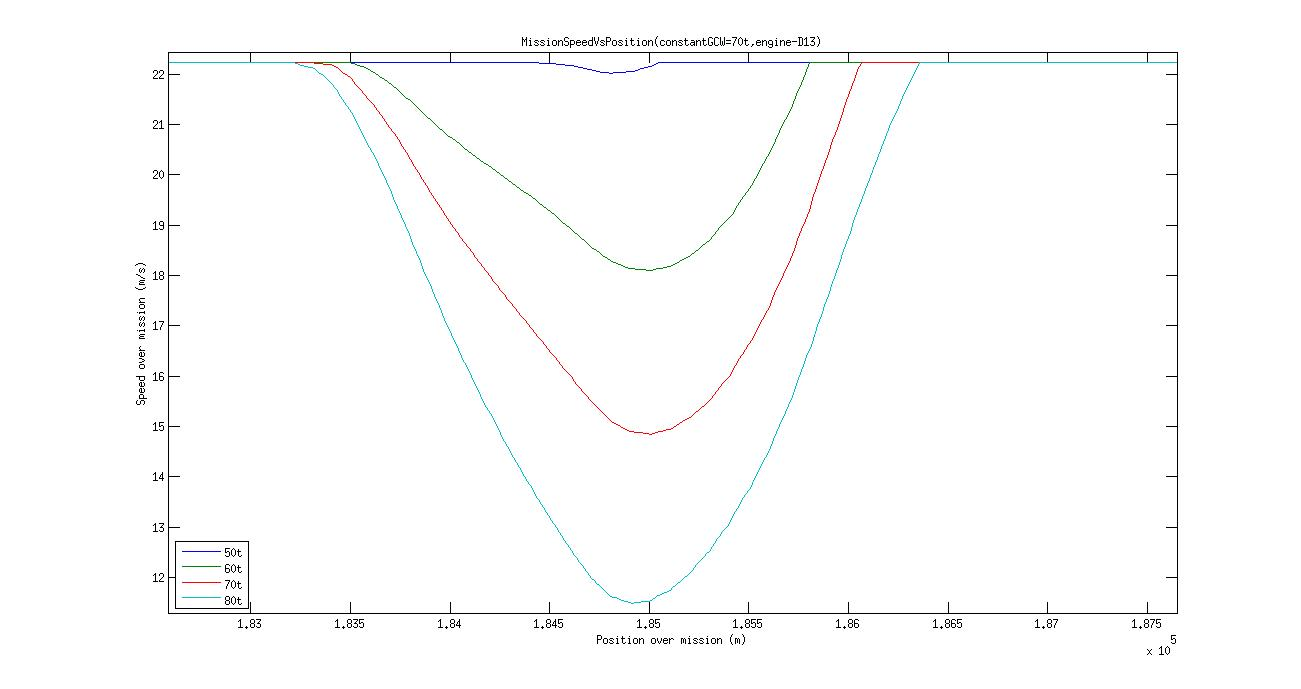
\includegraphics[width=\linewidth]{figures/ModelValidation/PlotsWithPredictiveControl/EngineSizeAndGCW/MissionSpeedZoomedInD13.jpg}
	\caption{Vehicle speed over mission, zoomed in at Hallands\aa sen - 011-010-01-010, D13, 70t}
	\label{speedZoomedEngineDownsizingPredictiveSoC}
	\end{figure}
	\subsection{Engine Size and Number of Axles Propelled}
	The anomalies in fuel consumption and mission time with increasing number of propelled axles when the non-predictive SoC management was used earlier (Figure \ref{timeFuelNumberOfAxlesEngine}) are seen to be decisively eliminated by the use of the predictive SoC strategy, as depicted in Figure \ref{timeFuelAxleEnginePredictiveSoC}.
	\begin{figure}
	\begin{subfigure}{.5\textwidth}
	\centering
	\includegraphics[width=\linewidth, clip=true, trim=45 185 55 208]{figures/ModelValidation/PlotsWithPredictiveControl/EngineSizeAndNoOFAxles/FuelConsumptionVsAxleNumberAndEngineSize.pdf}
	\caption{Fuel consumption over mission}
	\end{subfigure}
	\begin{subfigure}{.5\textwidth}
	\centering
	\includegraphics[width=\linewidth, clip=true, trim=45 185 55 210]{figures/ModelValidation/PlotsWithPredictiveControl/EngineSizeAndNoOFAxles/MissionTimeVsAxleNumberAndEngineSize.pdf}
	\caption{Mission time}
	\end{subfigure}
	\caption{Effect of engine size and GCW on fuel consumption and mission time with predictive SoC control}
	\label{timeFuelAxleEnginePredictiveSoC}
	\end{figure}
	\begin{figure}
	\centering
	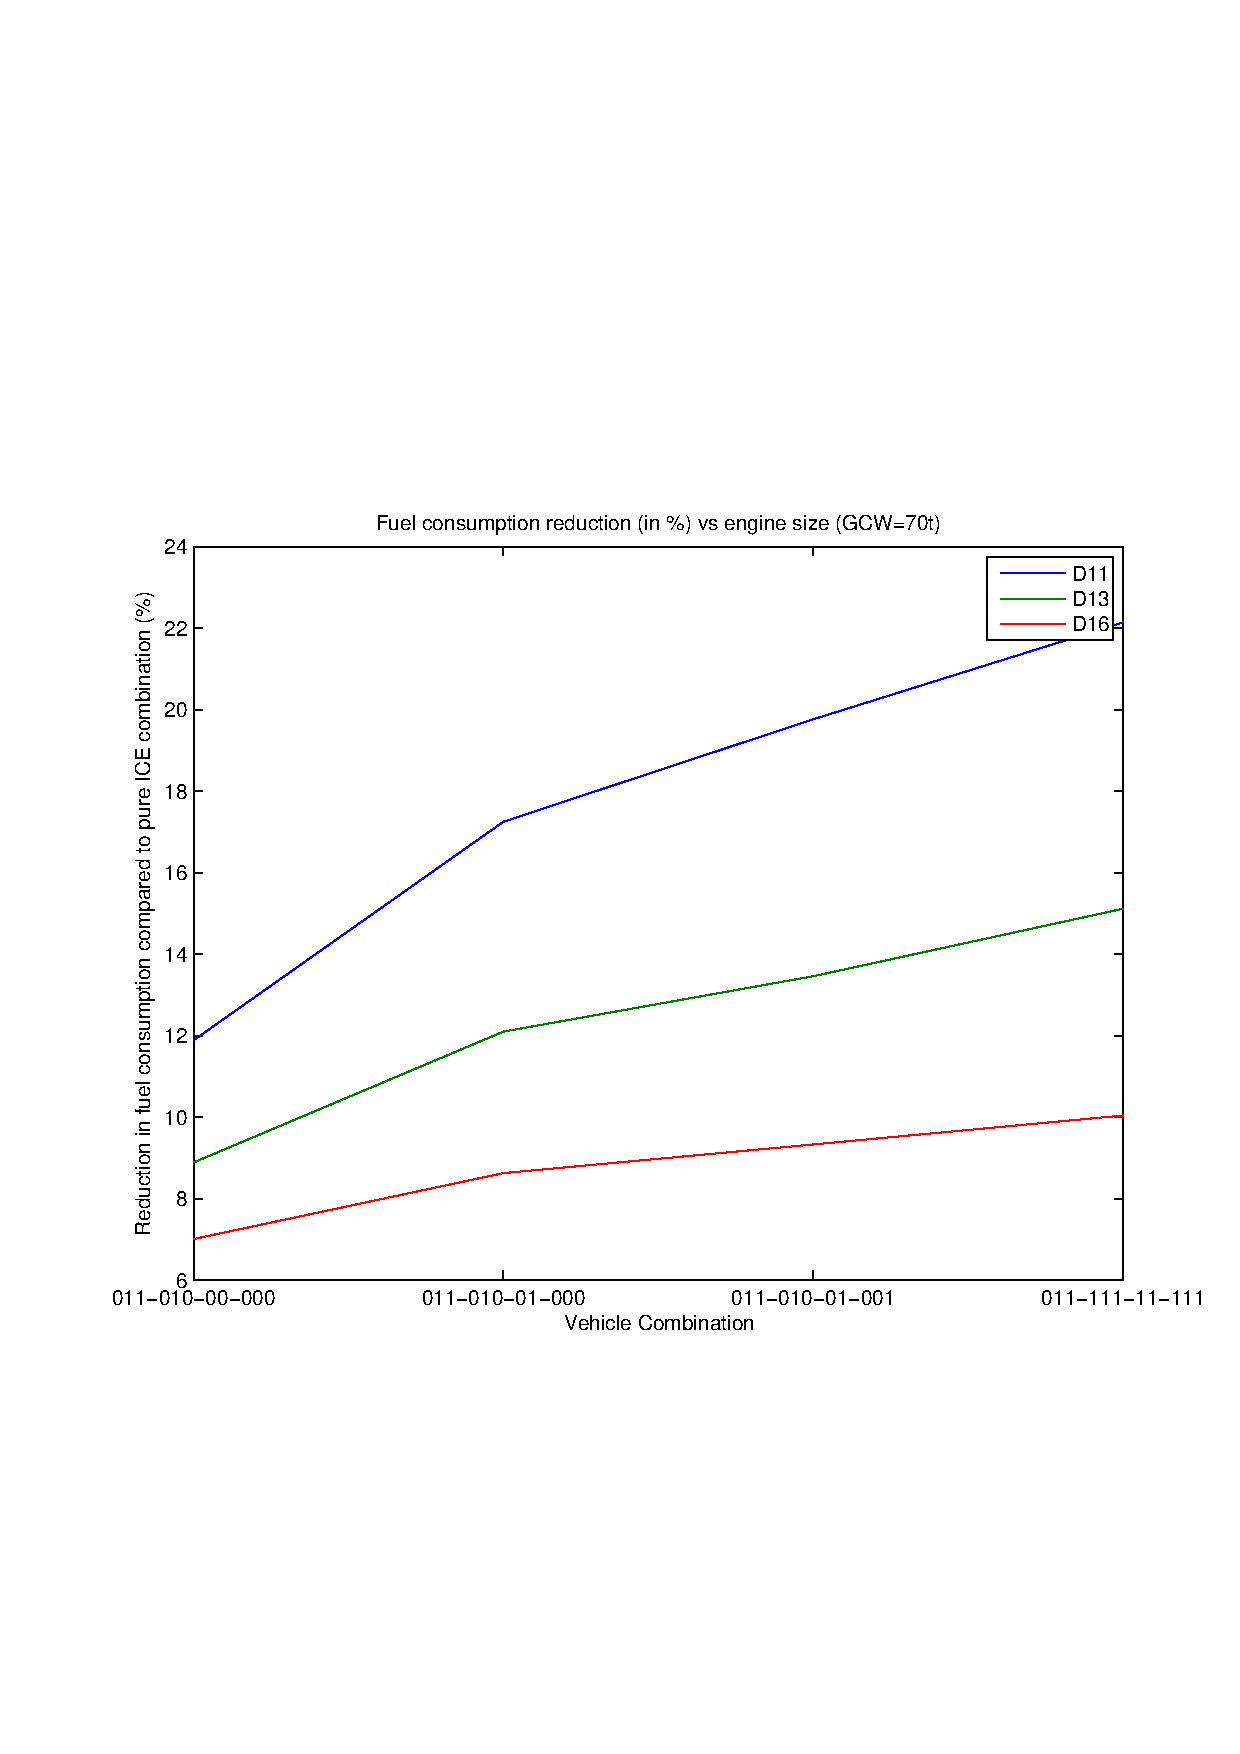
\includegraphics[width=0.5\linewidth, clip=true, trim=45 185 55 210]{figures/ModelValidation/PlotsWithPredictiveControl/EngineSizeAndNoOFAxles/FuelConsumptionReductionVsAxleNumberAndEngineSize.pdf}
	\caption{Reduction in fuel consumption compared to the pure ICE combination 011-000-00-000}
	\label{fuelReductionAxleEnginePredictiveSoC}
	\end{figure}
	\begin{figure}
	\centering
	\includegraphics[width=0.5\linewidth, clip=true, trim=45 185 55 210]{figures/ModelValidation/PlotsWithPredictiveControl/EngineSizeAndNoOFAxles/MissionSpeedVsPosition(constantGCW=70t,engine-D13).pdf}
	\caption{Mission speed for combinations with D13 engine, 70t GCW and varying levels of propulsion}
	\label{globalMissionSpeedIncreasedPropulsionPredictiveSoC}
	\end{figure}
	\begin{figure}
	\centering
	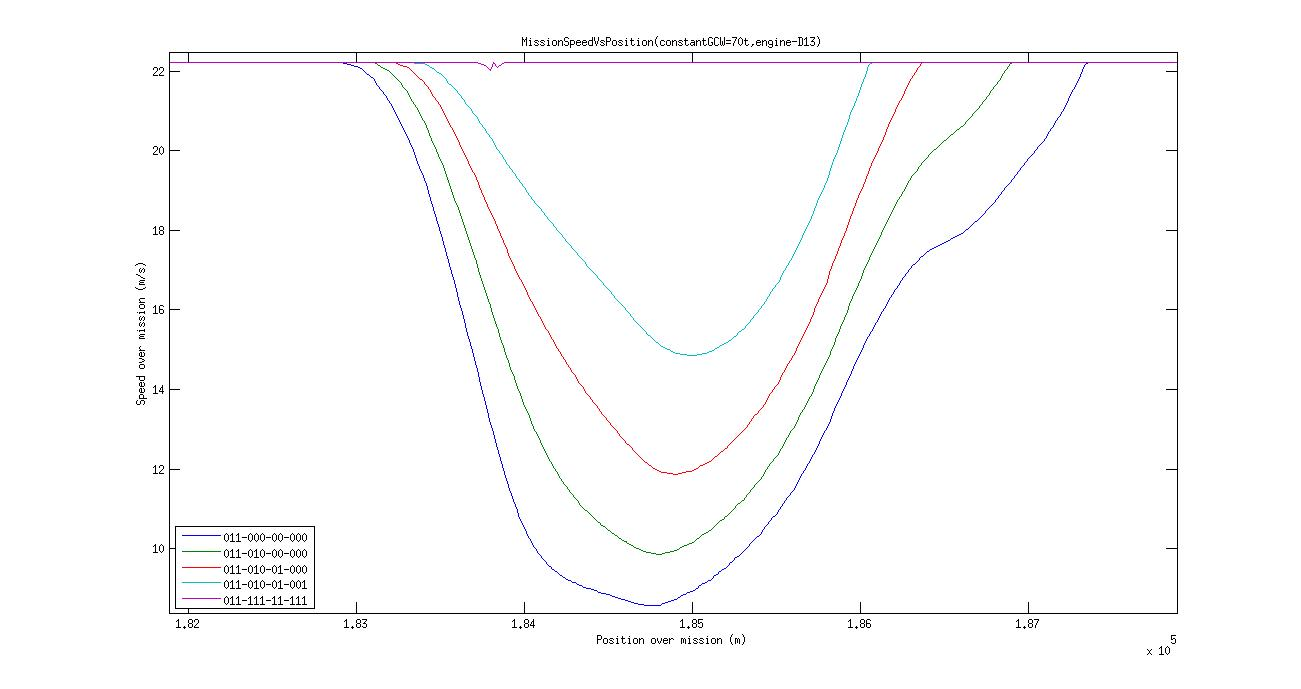
\includegraphics[width=\linewidth]{figures/ModelValidation/PlotsWithPredictiveControl/EngineSizeAndNoOFAxles/MissionSpeedZoomedIn.jpg}
	\caption{Mission speed at Hallands\aa sen, zoomed in - with fully predictive SoC management}
	\label{missionSpeedZoomedInIncreasedPropulsionPredictiveSoC}
	\end{figure}
	The percentage reduction in fuel consumption thus shows clear trends with engine size and axle configuration as seen in Figure \ref{fuelReductionAxleEnginePredictiveSoC}. The effect of the predictive SoC management can be seen far more clearly in the mission speed trends with increasing number of propelled axles. Figure \ref{globalMissionSpeedIncreasedPropulsionPredictiveSoC} shows the variation in vehicle speed over the mission for combinations with the D13 engine, GCW of 70t and varying levels of propulsion. Figure \ref{missionSpeedZoomedInIncreasedPropulsionPredictiveSoC} shows clear gradation in the minimum speed reached at the peak of Hallands\aa sen.

	\subsection{Buffer Size}
	The choice of the buffer size, in unison with the SoC control strategy determines the amount of charge consumed along the mission, thereby influencing vehicle mission productivity. Thus, four different vehicle propulsion configurations are simulated with varying (discrete) buffer sizes and their electrical energy consumptions compared. It must be borne in mind that these comparisons cannot be directly extrapolated to trends in mission productivity. They nevertheless yield an insight into the mechanism of the buffer size influence on overall combination charge consumption. The fuel and electrical energy consumption characteristics are as shown in Figure \ref{fuelElectricalEnergyBufferSizePredictiveSoC}.\\
	\begin{figure}
	\begin{subfigure}{.5\textwidth}
	\centering
	\includegraphics[width=\linewidth, clip=true, trim=45 185 55 208]{figures/ModelValidation/PlotsWithPredictiveControl/BufferSize/FuelConsumptionVsBufferSize.pdf}
	\caption{Fuel consumption over mission}
	\end{subfigure}
	\begin{subfigure}{.5\textwidth}
	\centering
	\includegraphics[width=\linewidth, clip=true, trim=45 185 55 210]{figures/ModelValidation/PlotsWithPredictiveControl/BufferSize/ElectricalEnergyConsumptionVsBufferSize.pdf}
	\caption{Mission time}
	\end{subfigure}
	\caption{Effect of buffer size and axle propulsion configuration on fuel consumption and mission time with full predictive SoC control}
	\label{fuelElectricalEnergyBufferSizePredictiveSoC}
	\end{figure}
	\section{Non-predictive pre-set varying depths of discharge along the mission}
	As an intermediate approach to the non-predictive and fully predictive SoC management strategies, a pre-determined lower SoC limit profile was developed based roughly of gradients encountered in each section of the mission. The performance of four different vehicle combinations was compared with those with the fully predictive SoC control in order to establish the efficacy of the latter. The SoC profile developed can be seen in Figure \ref{stepSoC}.\\
	\begin{figure}
	\centering
	\includegraphics[width=0.6\linewidth, clip=true, trim=45 185 55 210]{figures/ModelValidation/PlotsWithStepPredictiveControl/StepSoC.pdf}
	\caption{Buffer SoC Lower limit vs longitudinal position}
	\label{stepSoC}
	\end{figure}
	\begin{figure}
	\begin{subfigure}{.5\textwidth}
	\centering
	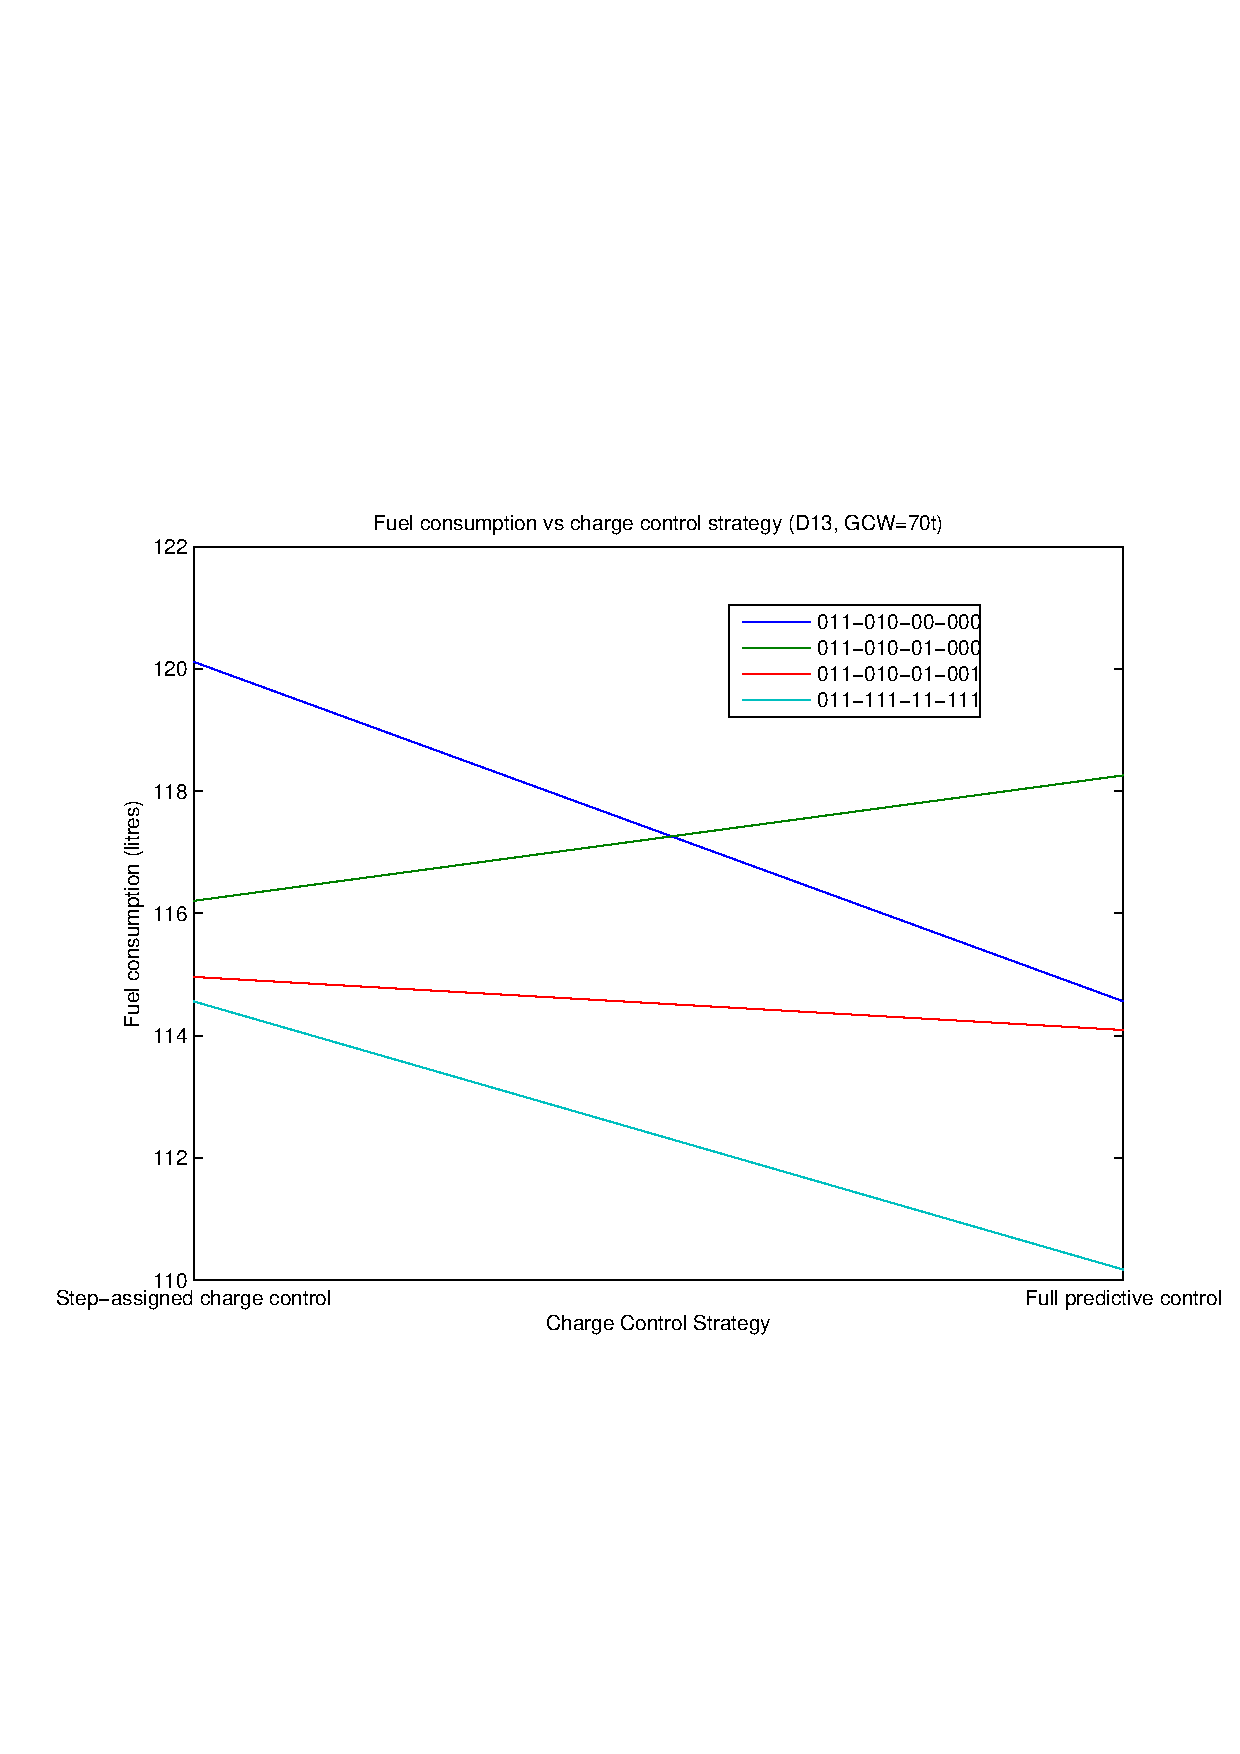
\includegraphics[width=\linewidth, clip=true, trim=45 185 55 208]{figures/ModelValidation/PlotsWithStepPredictiveControl/FuelConsumption.pdf}
	\caption{Fuel consumption over mission}
	\end{subfigure}
	\begin{subfigure}{.5\textwidth}
	\centering
	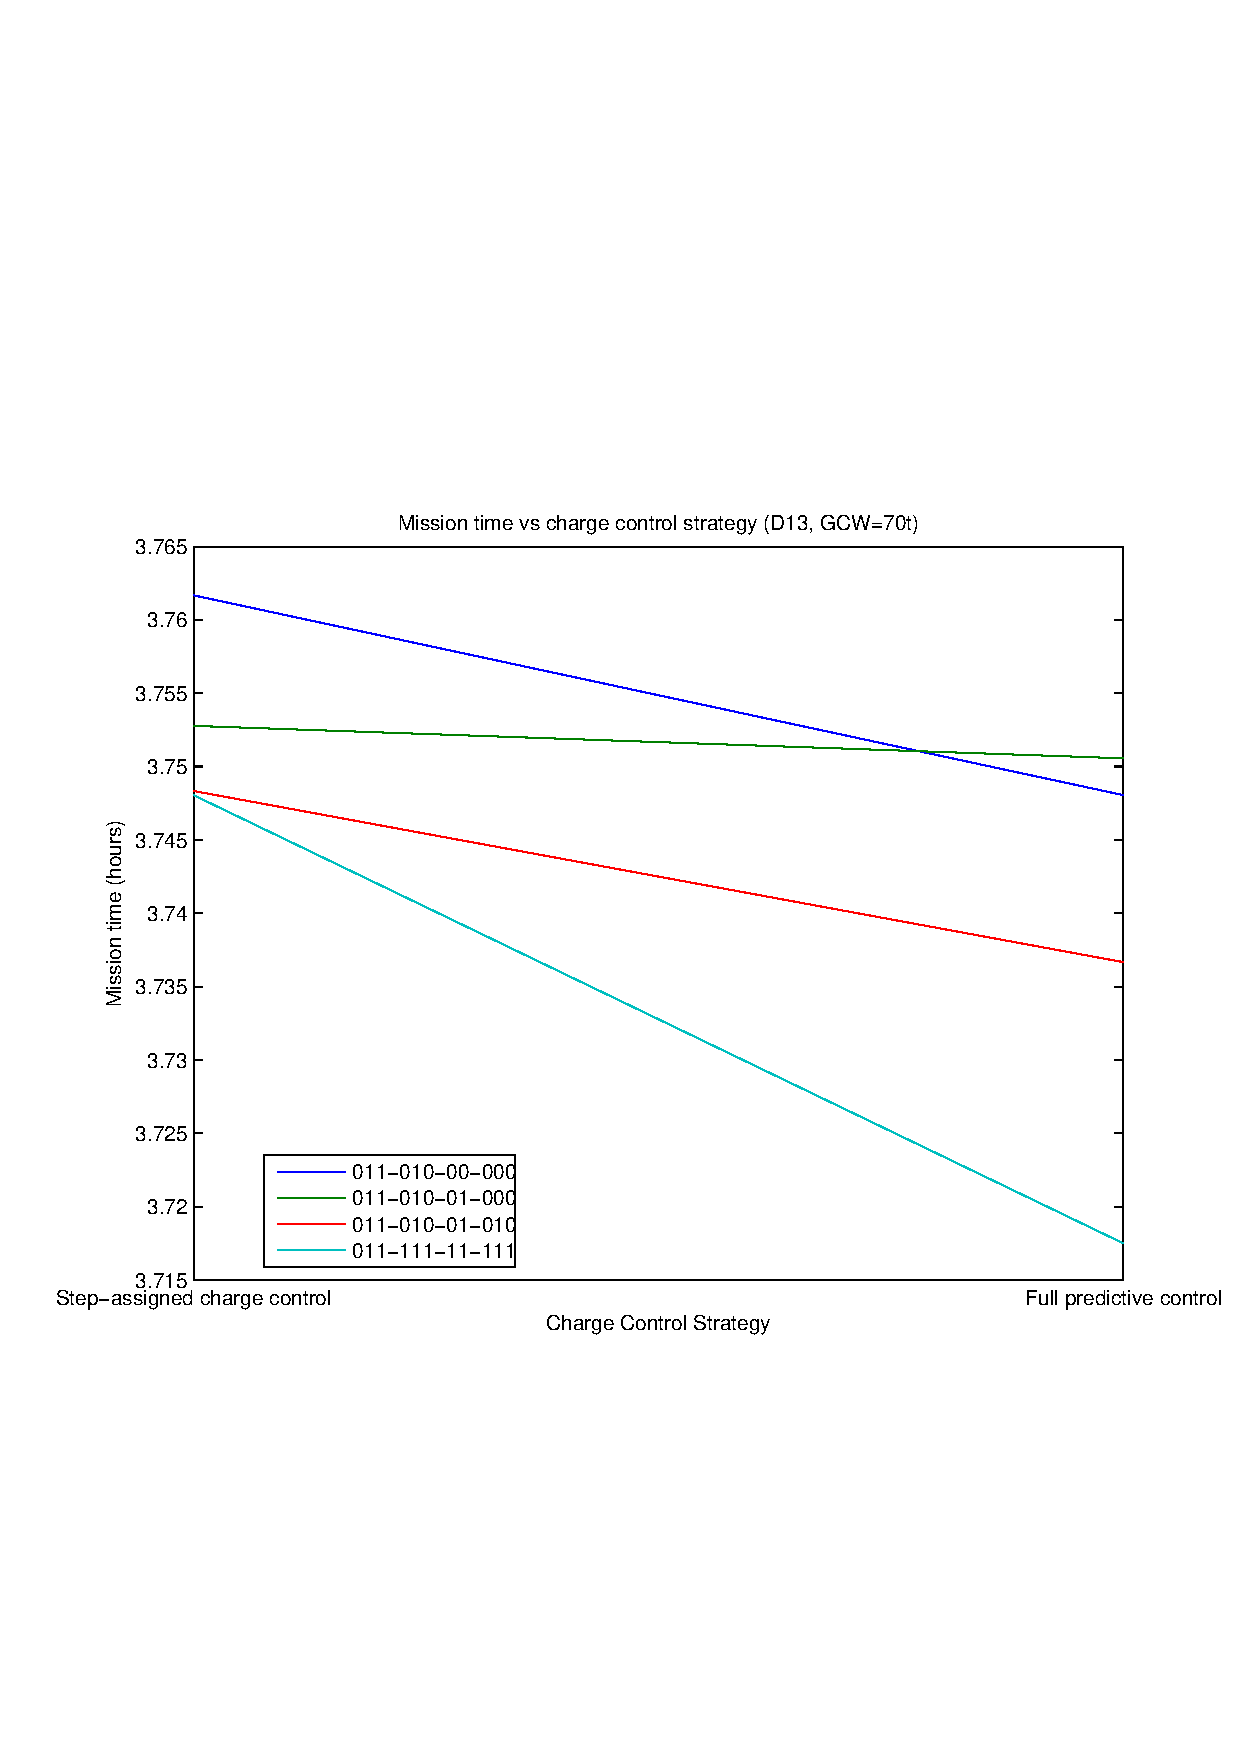
\includegraphics[width=\linewidth, clip=true, trim=45 185 55 210]{figures/ModelValidation/PlotsWithStepPredictiveControl/MissionTime.pdf}
	\caption{Mission time}
	\end{subfigure}
	\caption{Effect of engine size and GCW on fuel consumption and mission time with full and partial predictive SoC control}
	\label{timeFuelAxleEngineStepSoC}
	\end{figure}

	\begin{figure}
	\centering
	\includegraphics[width=0.6\linewidth, clip=true, trim=45 185 55 210]{figures/ModelValidation/PlotsWithStepPredictiveControl/ChargeConsumptionVsPosition1.pdf}
	\caption{Instantaneous electrical energy consumption vs longitudinal position}
	\label{electricalEnergyConsumptionStepSoC}
	\end{figure}

	The fully predictive SoC management favoured both fuel consumption and mission time as seen in Figure \ref{timeFuelAxleEngineStepSoC} as against the step-assigned SoC limits. Instantaneous electrical energy consumption was enhanced in the case of fully predictive control, as expected. The electrical energy consumption over the mission for the combination 011-010-00-000 with the D13 engine and 70t GCW is shown in Figure \ref{electricalEnergyConsumptionStepSoC}. The fully predictive SoC management controller is hence chosen to be used in all vehicle models utilised in the optimisation solver so as to obtain the ideal comparison between different vehicle propulsion configurations.

\end{document}
